Como se puede apreciar en el calendario (capítulo \ref{chp:calendario}), el
diseño de cada módulo que se integra en la aplicación se realizó en el ciclo
de desarrollo del propio módulo, una vez que se habían acordado con el cliente
las especificaciones detalladas en la sección \ref{sec:requisitos_funcionales}
y antes de comenzar la implementación, que se verá en el siguiente capítulo.

Al tratarse de una aplicación web, trataremos aspectos relacionados con el
código HTML que se mostrará al usuario, el diseño de la base de datos que dará
soporte a la aplicación, así como la arquitectura subyacente para guardar y
recuperar esos datos a través de la interfaz de usuario.

\section{Diseño de la interfaz de usuario}

La interfaz de usuario es la única parte de la que el usuario final va a ser
plenamente consciente, por lo que debe tratarse con suficiente detalle de
manera que no resulte demasiado confusa y no dé lugar a errores.

En la sección \ref{sec:requisitos_interfaz}, se indicó que el diseño de la
interfaz no debía ser uno de los principales focos de atención a la hora de
diseñar la herramienta. Se argumentó que el grupo de usuarios finales estaría
formado por personas con cierta soltura en el manejo de sistemas de gestión en
el ámbito de la empresa. Un principio básico que el proyectante tiene muy claro
es que «los usuarios pasan la mayor parte de su tiempo visitando otras
páginas»\footnote{«Jakob's Law of the Web User Experience states that ``users
spend most of their time on other websites.''». Fuente:
\href{http://www.useit.com/alertbox/9605.html}{
http://www.useit.com/alertbox/9605.html}.}, por lo que es importante seguir las
convenciones establecidas.

En las próximas páginas, se mostrarán los ejemplos más representativos de las
decisiones tomadas en el contexto del diseño de la interfaz.

\subsection{Generalidades}

La interfaz está parcialmente definida por la herramienta de objetivo general en
la que se integraría este desarrollo. Es por ello que se realizó un esfuerzo
para mantener la homogeneidad visual de modo que el usuario no sintiese que se
estaba enfrentando a una herramienta totalmente desligada del resto. Para ello,
el proyectante solo debía conocer someramente el código de las pantallas
existentes y familiarizarse con la hoja de estilos CSS que se había usado. Esto
fue muy sencillo, ya que entre las labores que el proyectante realizó durante su
periodo de prácticas antes de centrarse este proyecto en cuestión, estaba
precisamente la de reformar su apariencia visual, como se hizo constar en la
introducción de esta memoria (sección \ref{sec:antecedentes}).

Debe destacarse que no se realizaron diseños previos más allá de bocetos
manuscritos elaborados en colaboración con el cliente. Una vez reunidos los
bocetos, que ayudaban a revisar que las especificaciones serían capaces de
cumplir con lo que el cliente quería encontrarse finalmente en la pantalla, se
llevó a cabo la labor de programación para, finalmente, construir la interfaz
de usuario. La estrecha colaboración con el cliente hizo posible introducir,
sobre la marcha y de forma muy ágil, cualquier modificación sobre el producto
final.

\subsection{Formularios}

\begin{figure}
\centering
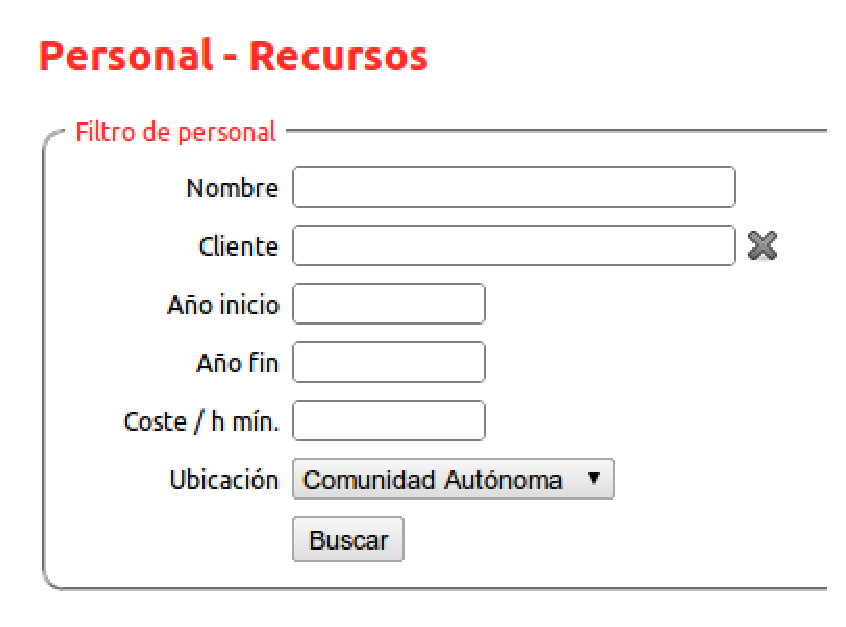
\epsfig{file=imagenes/filtro_personal.eps,width=3.5in}
\caption{Detalle del filtro de personal.}
\label{fig:detalle_filtro_personal}
\end{figure}

En las especificaciones, se ha insistido en la necesidad de facilitar al máximo
la labor de búsqueda de información. La imagen \ref{fig:detalle_filtro_personal}
muestra un detalle del filtro de personal. Se aprecia el uso de cajas de texto
para casi todos los campos, exceptuando la caja de selección de Comunidad
Autónoma. Podría argumentarse que la selección de cliente también es susceptible
de implementarse por medio de una caja de selección, pero se tomó la decisión de
crear un sistema de sugerencias para la selección de clientes, implementado
haciendo uso de AJAX, como se verá en el capítulo \ref{chp:implementacion}. La
motivación para esta decisión no es otra que el elevado y creciente número de
clientes de Ingeniería e Innovación. A fecha de creación de esta memoria, el
número de clientes registrados es de 214, por lo que el uso de una caja de
selección típica resulta demasiado pesado para el usuario, que se vería forzado
a navegar por la lista cada vez que quisiera seleccionar un cliente. La barra de
desplazamiento de la imagen \ref{fig:seleccion_cliente_old} (difuminada
intencionadamente) puede dar una idea
de lo larga que es esa lista y la incomodidad que puede causar al usuario.

\begin{figure}
\centering
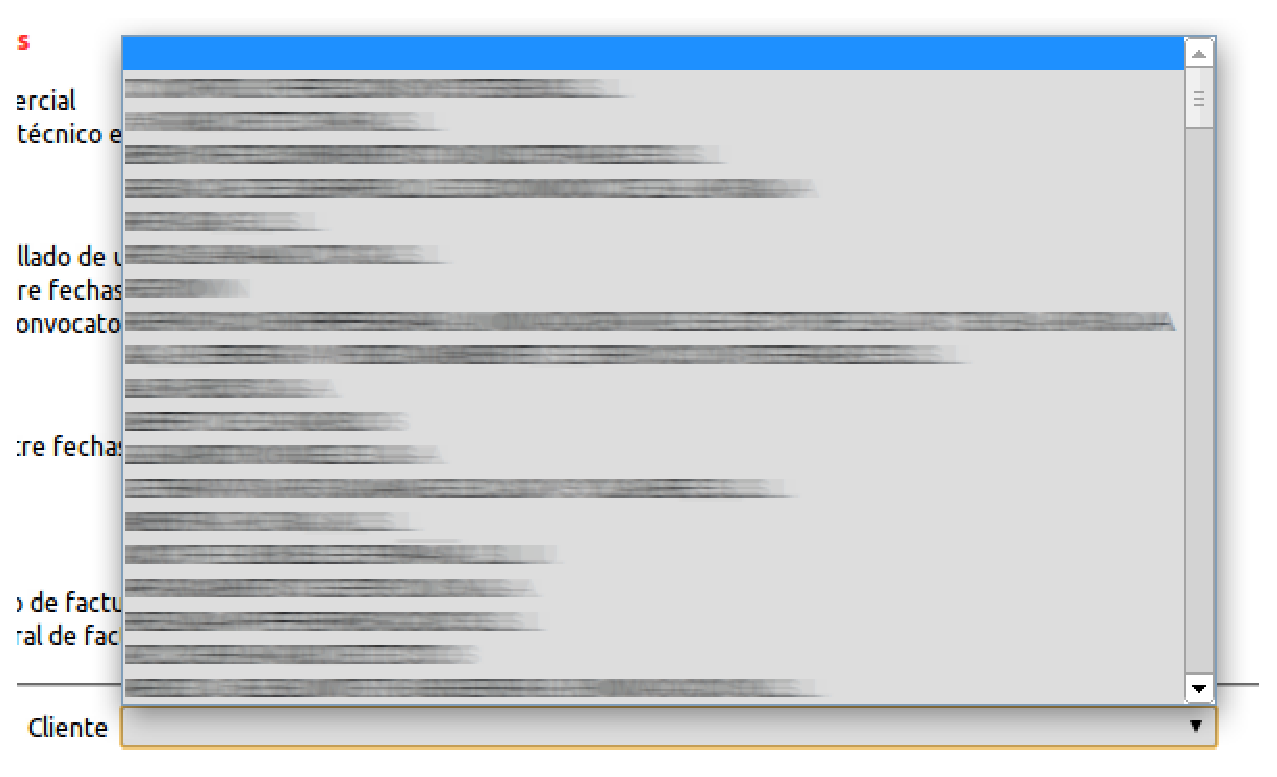
\epsfig{file=imagenes/seleccion_cliente_old.eps,width=5in}
\caption{Selección de cliente mediante caja de selección.}
\label{fig:seleccion_cliente_old}
\end{figure}

El enfoque de las sugerencias, que se usará también en la selección de
proyectos (392 hasta el momento y creciendo), está cada vez más presente en muy
diversos ámbitos de la web (sirva como ejemplo la figura
\ref{fig:sugerencias_web}), ya que ofrece varias ventajas respecto al otro
sistema:

\begin{itemize}
 \item Elimina la necesidad de mostrar toda la lista, que es muy grande y
podría ralentizar la descarga de la página.
 \item Facilita y acelera la búsqueda: cuando el usuario ha introducido tres o
cuatro letras, ya obtiene los resultados esperados.
 \item Es muy versátil: en el caso de los proyectos,
el usuario puede buscarlos por nombre, acrónimo, cliente y acrónimo de cliente.
\end{itemize}


\begin{figure}
\centering
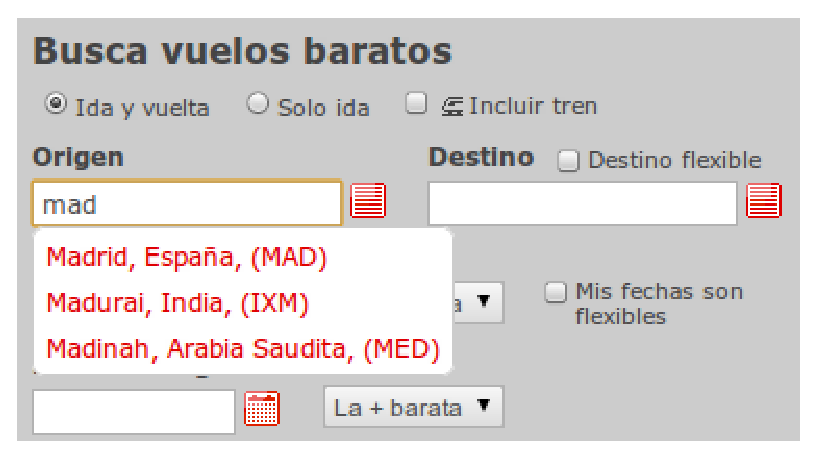
\epsfig{file=imagenes/sugerencias_web.eps,width=3in}
\caption{Sugerencias de aeropuerto en un portal de vuelos.}
\label{fig:sugerencias_web}
\end{figure}

Los formularios están creados usando las mismas estructuras que los ya
existentes, de modo que la experiencia es siempre la misma. La figura
\ref{fig:comparacion_formularios} muestra una comparación entre un formulario
nuevo y uno ya existente.

\begin{figure}
\centering
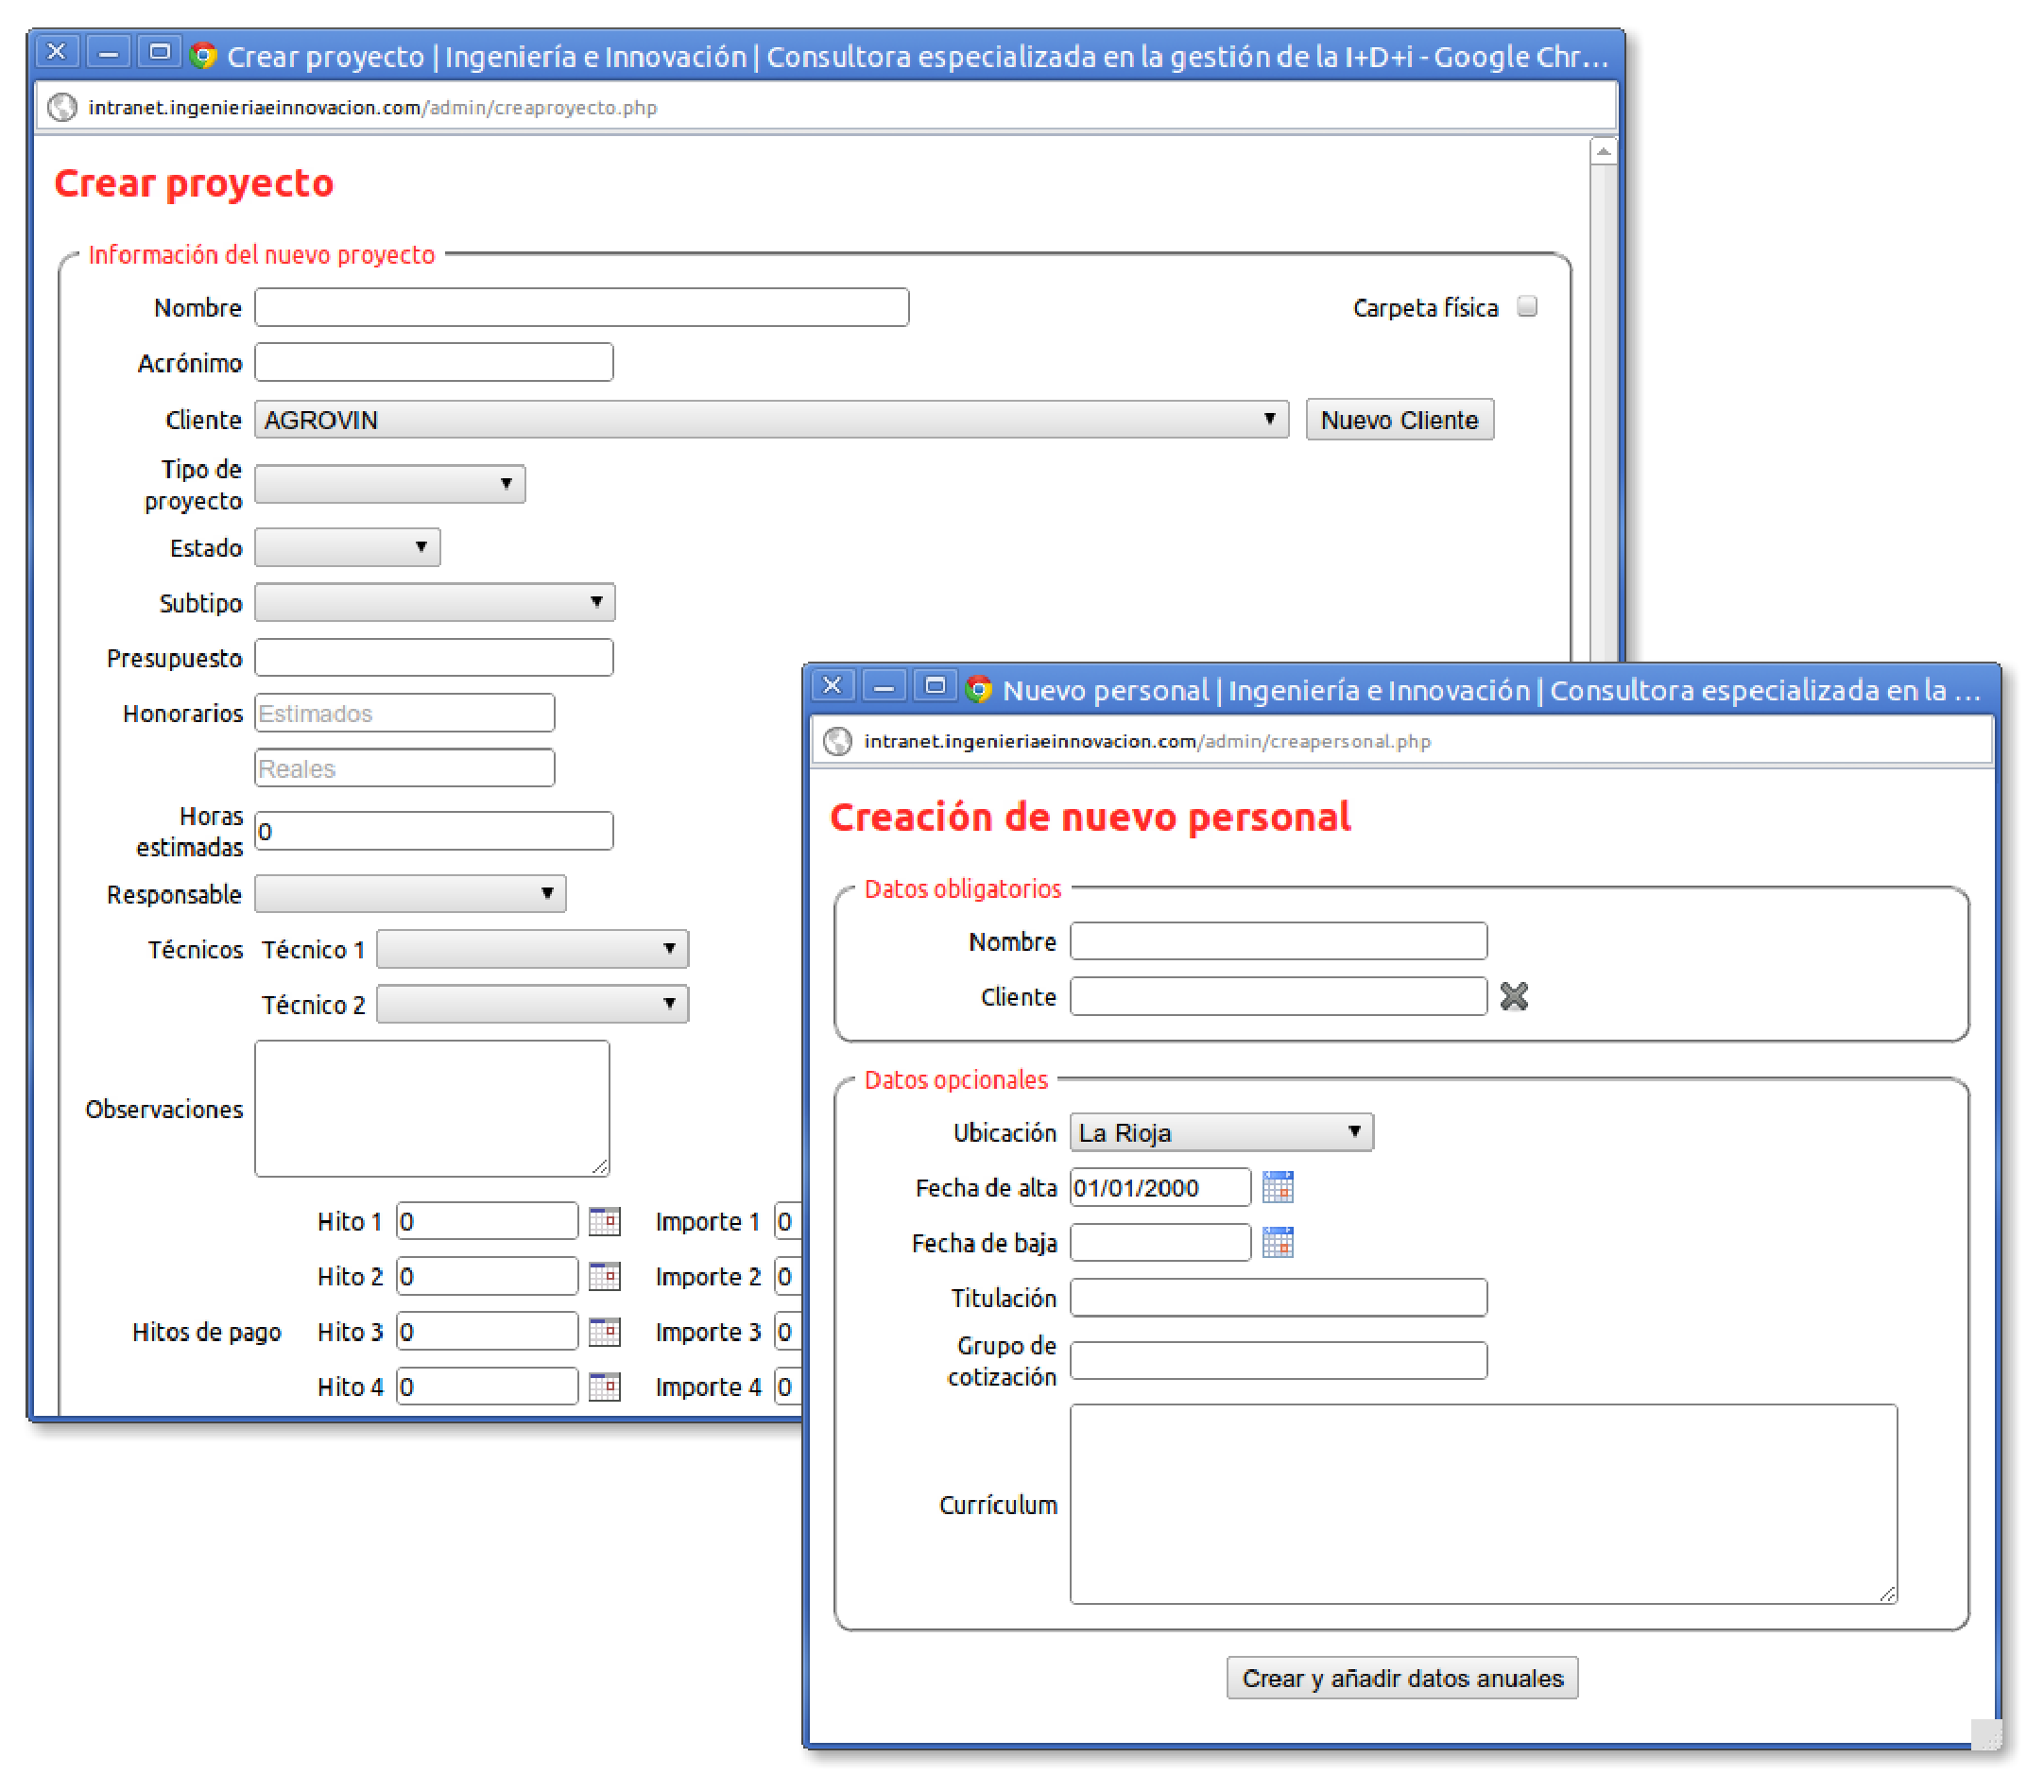
\epsfig{file=imagenes/comparacion_formularios.eps,width=5.28in}
\caption{Formulario existente (izq.) frente a formulario nuevo (dcha.).}
\label{fig:comparacion_formularios}
\end{figure}

En la figura \ref{fig:comparacion_formularios} puede apreciarse otra decisión
tomada en favor de la usabilidad de la interfaz: en lugar de marcar los campos
obligatorios en negrita o con un asterisco, estos se encuentran
físicamente separados en su propio \textit{fieldset} con la etiqueta «Datos
obligatorios».

\subsection{Tablas}

La herramienta está plagada de tablas: se usan para mostrar los registros
anuales de los recursos humanos, para mostrar las actividades de cada proyecto,
en el detalle mensual de horas...

En la figura \ref{fig:tablas} se comprueba que se han intentado tratar de
la misma manera, para que la experiencia sea consistente.

\begin{figure}
\centering
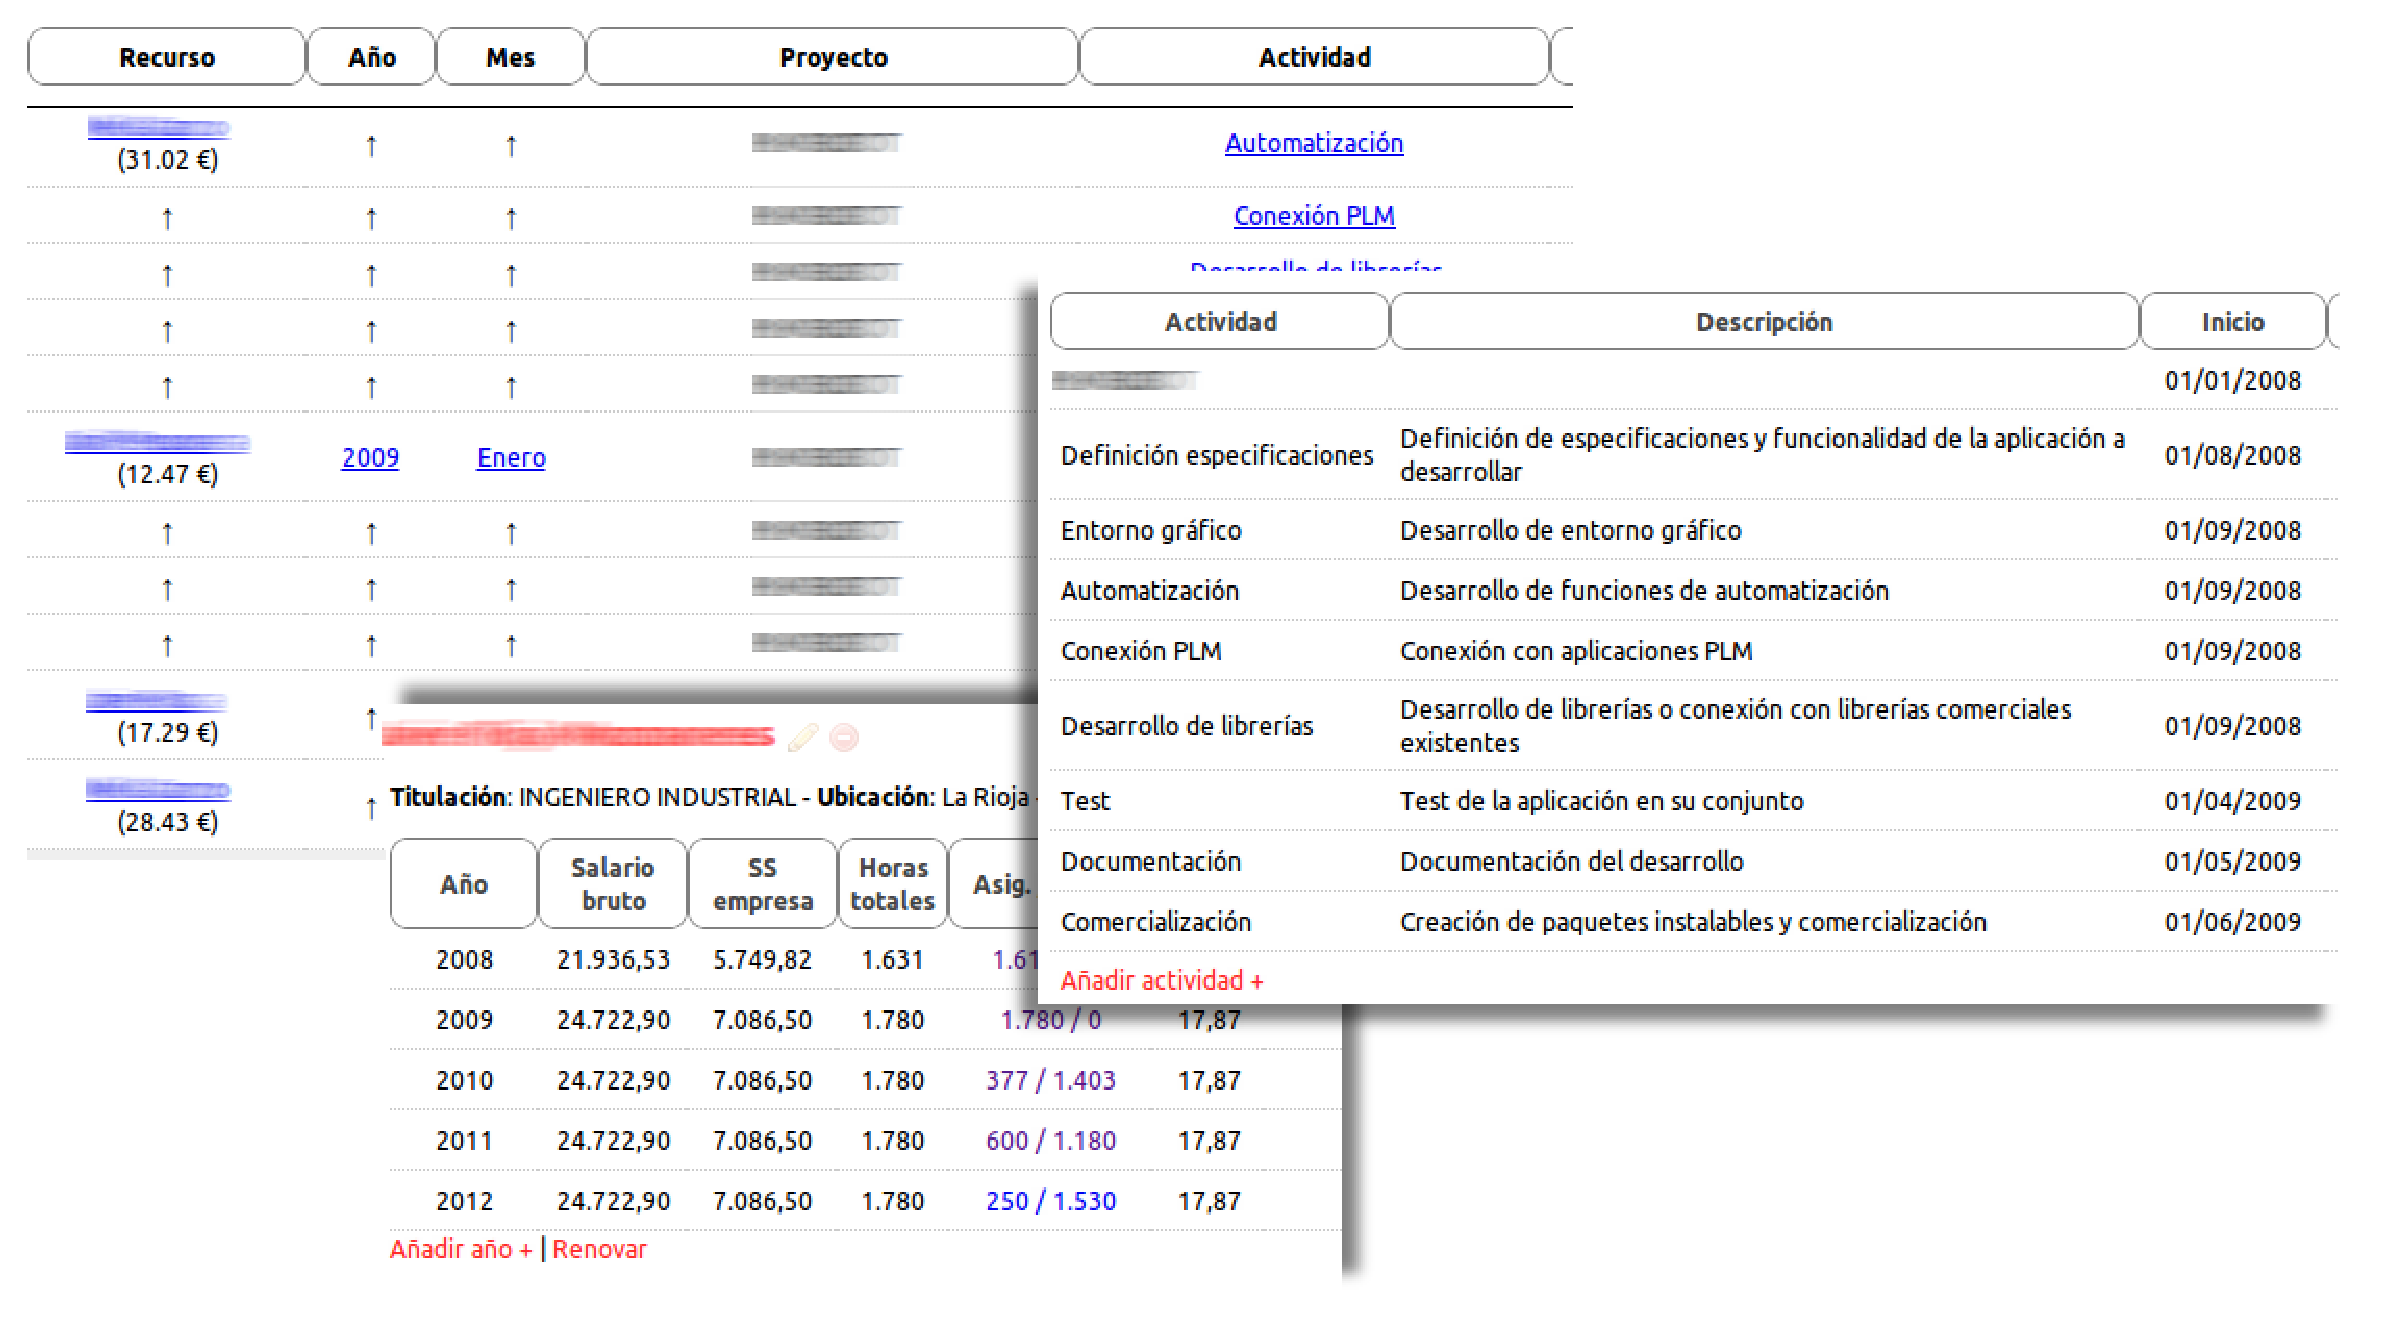
\epsfig{file=imagenes/tablas.eps,width=5.28in}
\caption{Varias tablas de la herramienta.}
\label{fig:tablas}
\end{figure}

Una característica interesante es que se ha incluido en las tablas la capacidad
de ordenarlas pinchando en la cabecera de cada columna, al estilo de las
aplicaciones de escritorio. En el capítulo \ref{chp:implementacion} se hará
referencia a esta cualidad, lograda por medio de una librería externa.

\begin{figure}
\centering
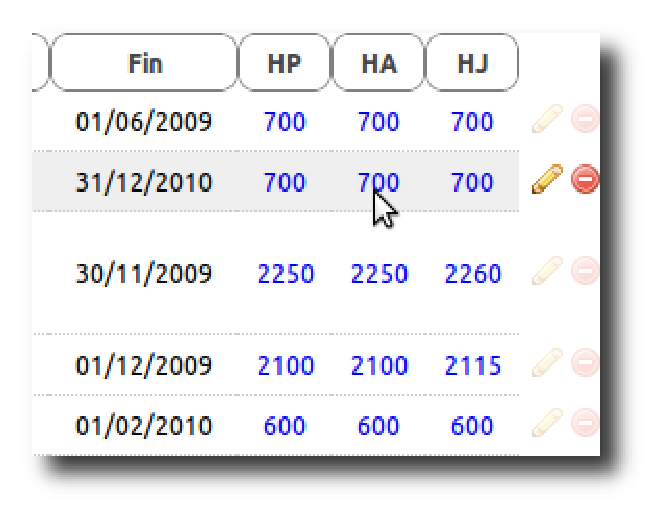
\epsfig{file=imagenes/detalle_tabla.eps,width=3in}
\caption{Detalle de fila activa en una tabla.}
\label{fig:detalle_tabla}
\end{figure}

También, como segunda decisión de importancia tomada acerca de las tablas, la
fila sobre la que está el cursor se resalta con un fondo gris y las opciones de
modificación, eliminación..., que son semitransparentes, se hacen opacas, como
se puede apreciar en la figura \ref{fig:detalle_tabla}.

Como se puede ver en las imágenes mostradas, se ha intentado que
las tablas sean limpias y claras mostrando únicamente los bordes inferiores de
cada fila, evitando el uso de \textit{colspans} y, en general, evitando el uso
de tablas para datos que no sean tabulares, en contraposición a otras tablas
presentes en la aplicación global, que han demostrado ser confusas y difíciles
de mantener (ver figura \ref{fig:tabla_antigua}).

Finalmente, las tablas están llenas de enlaces: a detalles de horas,
información de recursos... En este sentido, se decidió no dar formato a los
enlaces, de modo que siguen la convención habitual, azules los no visitados,
morados los visitados. Los iconos, por su parte, están tomados de otras partes
de la aplicación global, para mantener la consistencia.

\begin{figure}
\centering
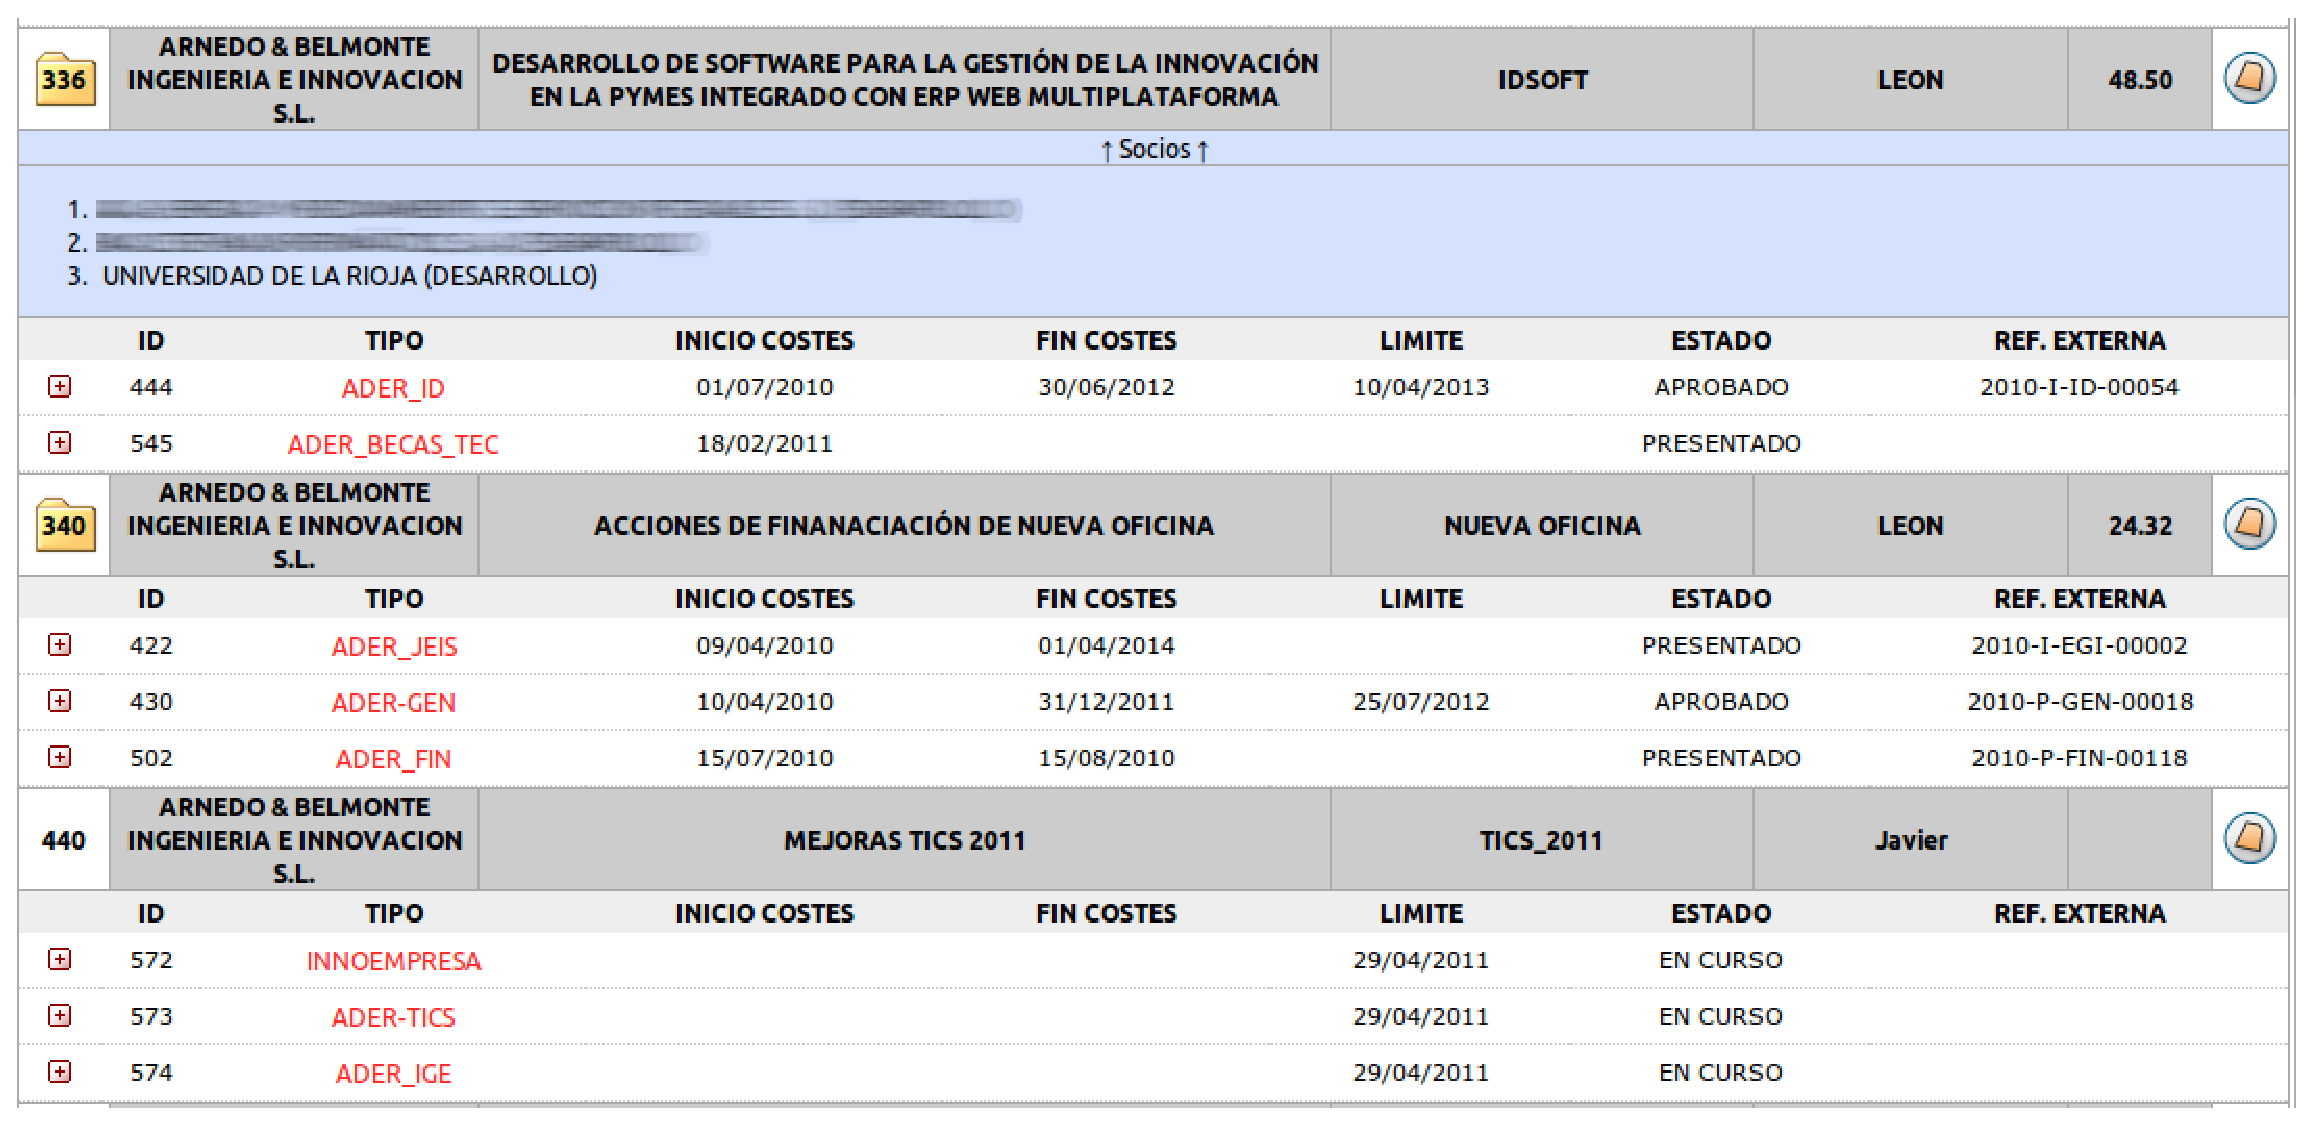
\epsfig{file=imagenes/tabla_antigua.eps,width=5.28in}
\caption{Tabla antigua.}
\label{fig:tabla_antigua}
\end{figure}

\subsection{Ventanas emergentes}

La interacción con la herramienta incluye multitud de ventanas emergentes, en
consonancia con las partes preexistentes: se usan para crear personal y
actividades, asignar horas, modificar entidades...

El proyectante, conocedor de la tendencia a prescindir de este tipo de
interacción a la hora de diseñar interfaces, ha probado el uso de
\textit{lightboxes} en otras partes de la aplicación menos relevantes, pero
hasta que no se tome la decisión de abandonar el método de las ventanas
emergentes de forma completa, se ha decidido seguir de esta manera.

Una ventaja de las ventanas emergentes es que muchas veces se necesita
información de la ventana previa para rellenar el formulario de
creación/modificación oportuno, y estas ventanas lo consiguen independizándose
totalmente. Sin embargo, rompen la tónica habitual de lo que debería ser una
experiencia fluida y muchos usuarios acaban teniendo infinidad de ventanas
emergentes porque no se dan cuenta de que ya tenían una y siguen abriendo. Las
\textit{lightboxes} son una clase muy particular de elemento dentro de la propia
página que centra la atención del usuario sin romper la experiencia, y en muchos
casos, dejando la mayor parte de la vista original visible (aunque a veces
atenuada para captar la atención del usuario), como se aprecia en la figura
\ref{fig:ventana_modal}.

\begin{figure}
\centering
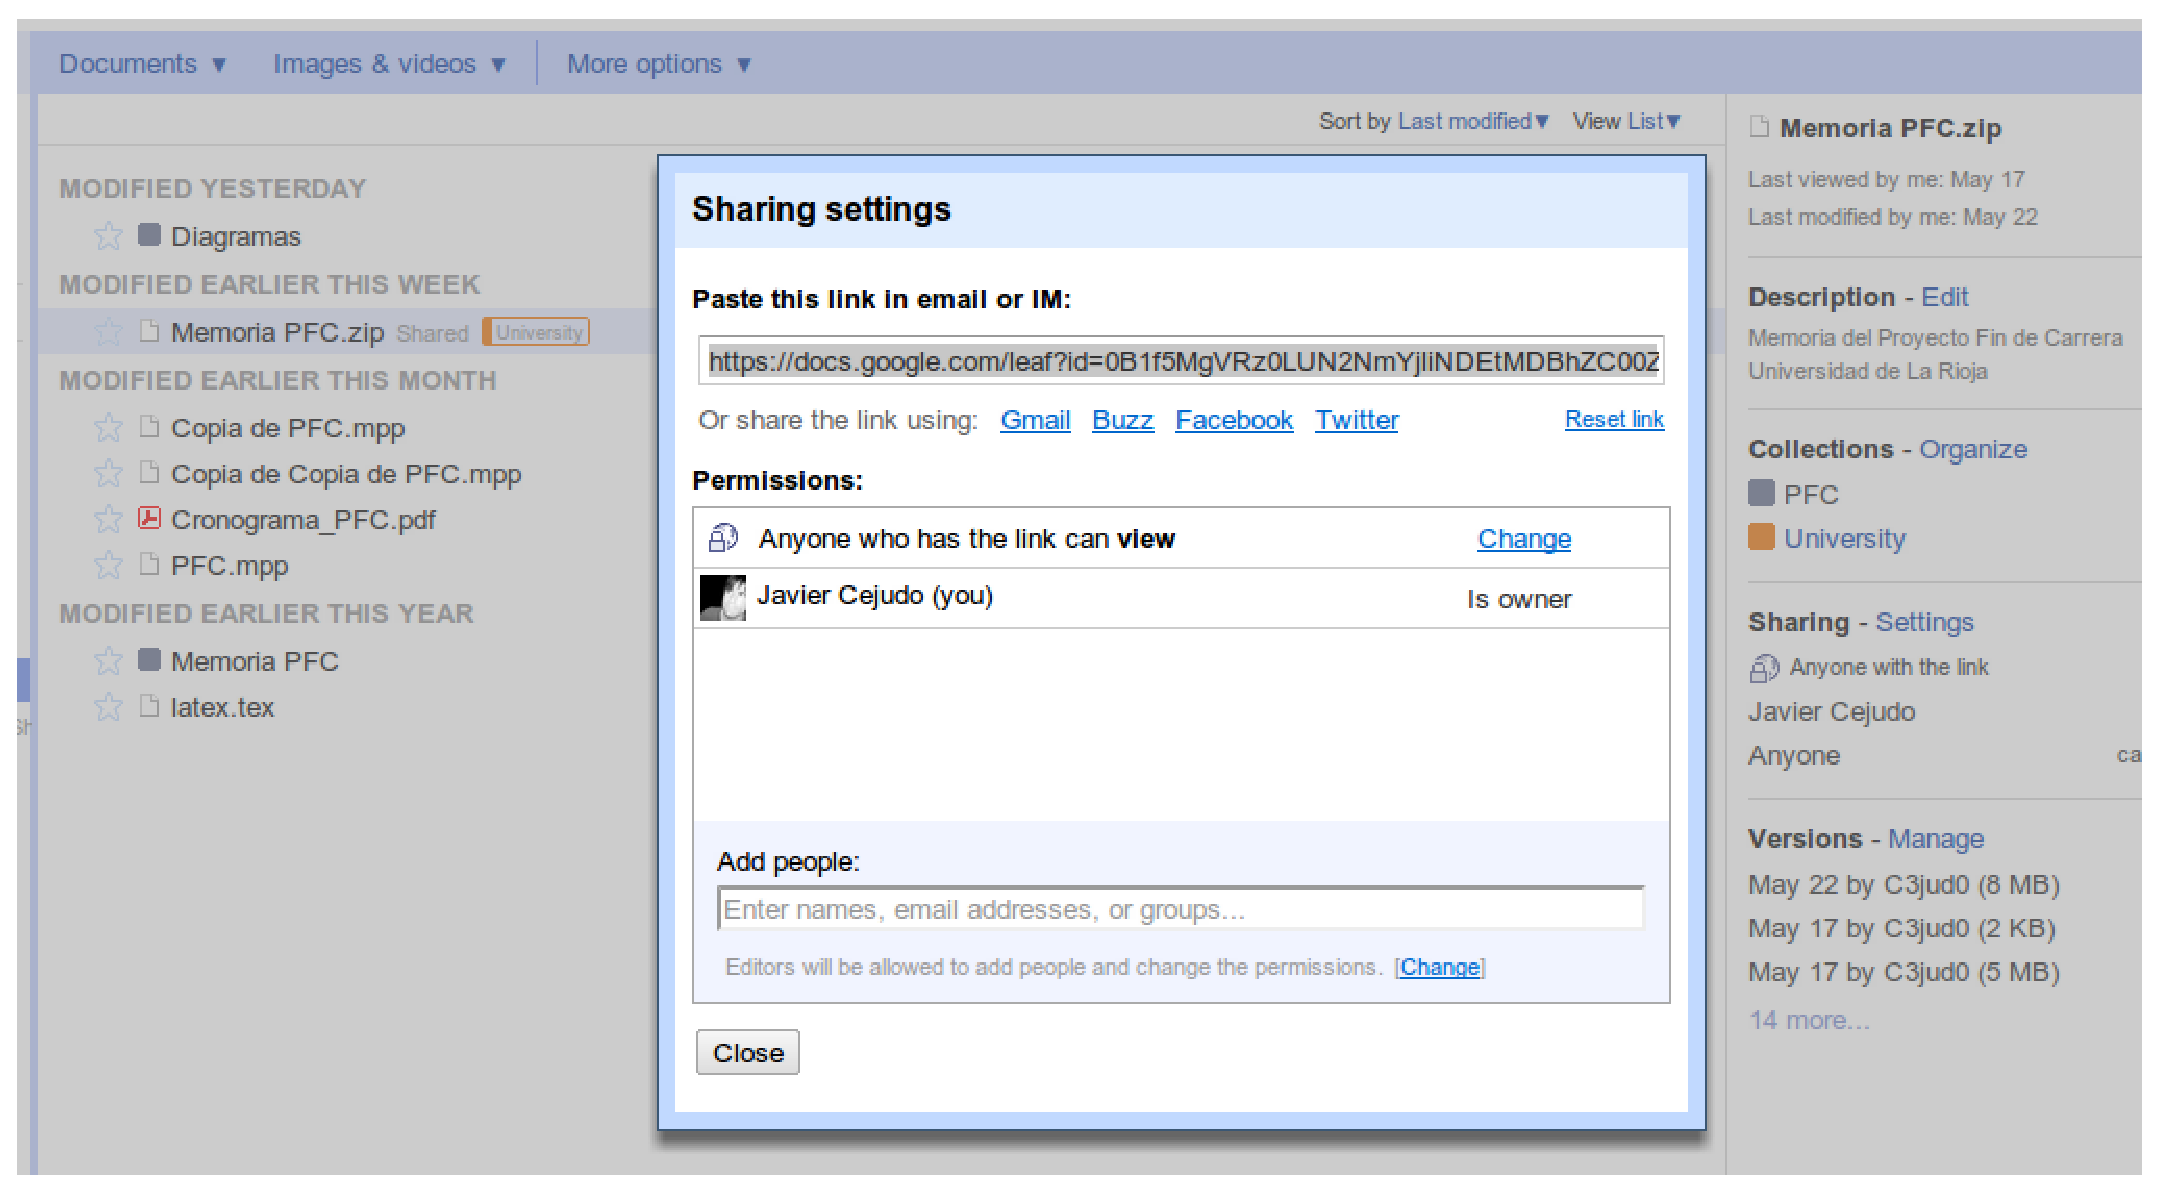
\epsfig{file=imagenes/ventana_modal.eps,width=5.28in}
\caption{Ejemplo de lightbox en Google Docs.}
\label{fig:ventana_modal}
\end{figure}

\subsection{Buscador global}

\begin{figure}
\centering
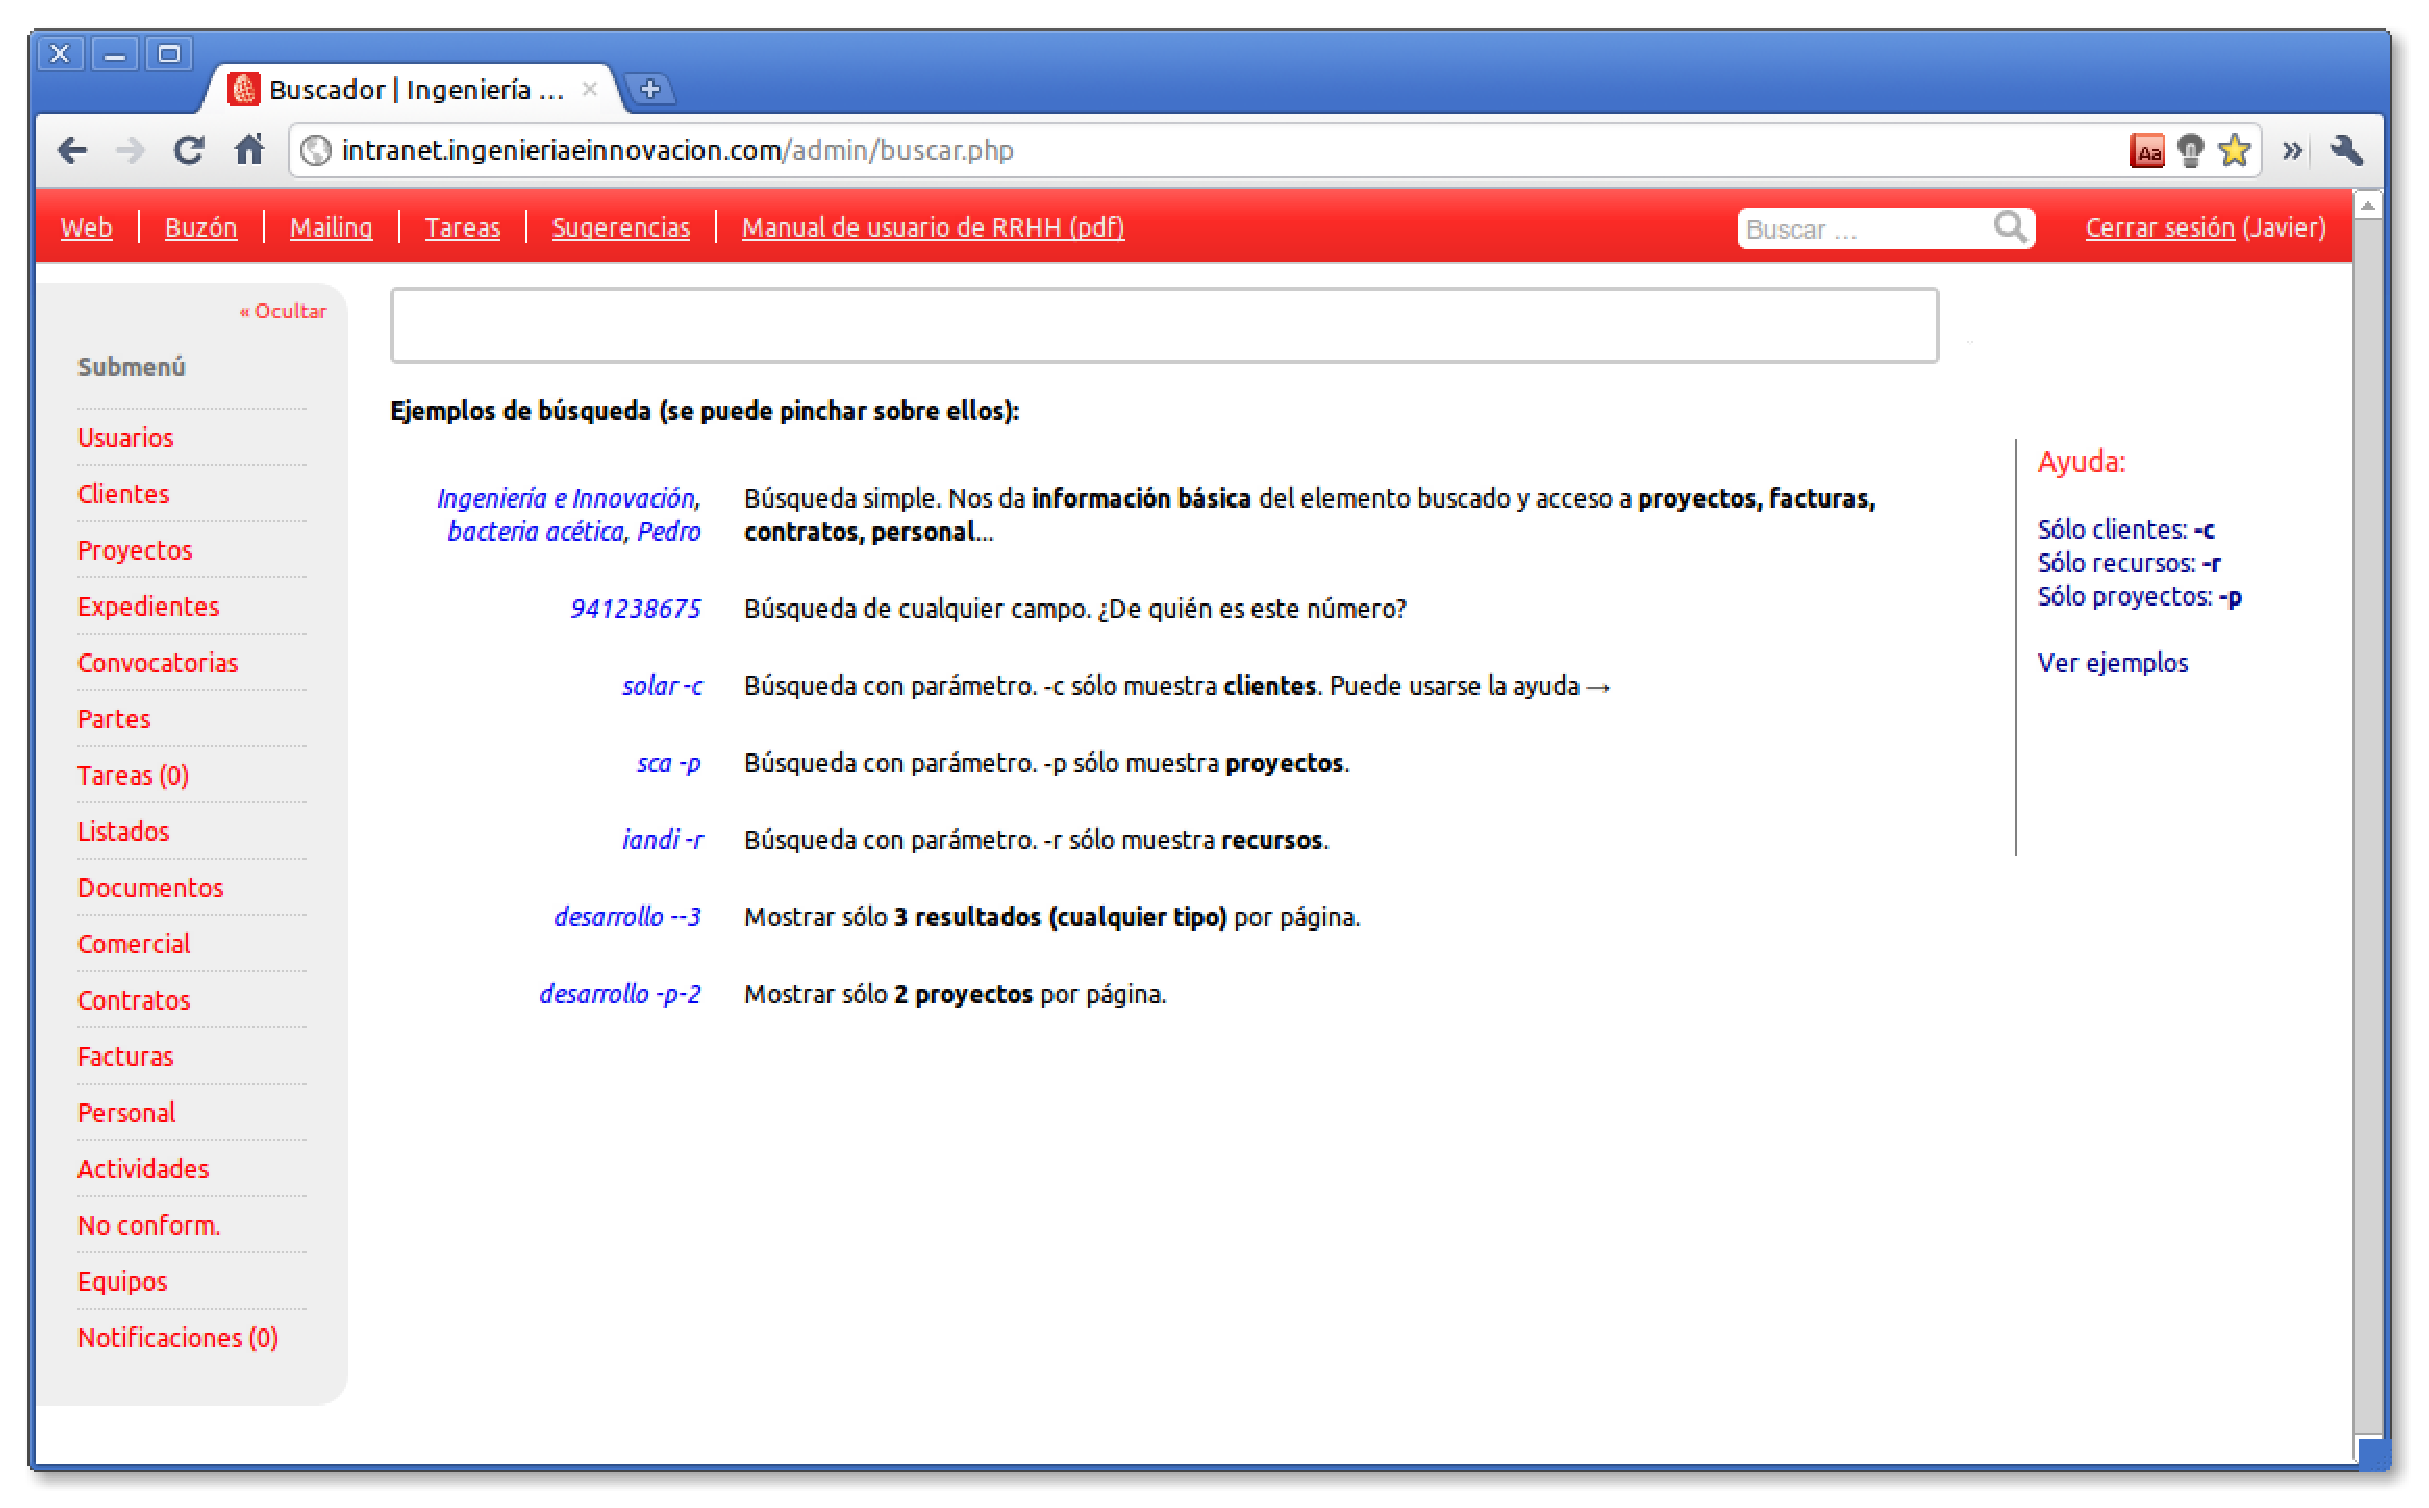
\epsfig{file=imagenes/buscador_inicio.eps,width=5.28in}
\caption{Buscador global.}
\label{fig:buscador_inicio0}
\end{figure}

El buscador, al ser una herramienta nueva y diferenciada del resto de la
aplicación, ha requerido un mayor número de decisiones de cara a su diseño.

En primer lugar, muestra una serie de ejemplos, desde los más simples hasta
ejemplos más avanzados, de modo que estén a mano en cualquier momento y los
usuarios se familiaricen con ellos. Estos ejemplos están brevemente explicados y
son interactivos, de manera que pinchando en ellos veremos el tipo de resultados
que proporcionan.

Los colores empleados son los corporativos, pero la estructura de los resultados
es muy similar a la de los buscadores generalistas (véase la figura
\ref{fig:resultado_busqueda}): título, descripción, datos adicionales y otros
enlaces de interés.

\begin{figure}
\centering

\epsfig{file=imagenes/resultado_busqueda.eps,width=5.28in}
\caption{Detalle de un resultado.}
\label{fig:resultado_busqueda}
\end{figure}

La paginación funciona, también, como en cualquier otro buscador: enlaces a las
páginas siguientes, a las anteriores, marcado de página actual, y enlace
siempre visible a la primera y última página, para dar contexto. Dada la
naturaleza instantánea del buscador, se han seguido las convenciones do Google
Instant: cada vez que el buscador está cargando, los resultados se vuelven
semitransparentes (figura \ref{fig:buscador_cargando}), y en el caso de cambio
de página, la barra de desplazamiento se posiciona al principio de los
resultados.

\begin{figure}
\centering
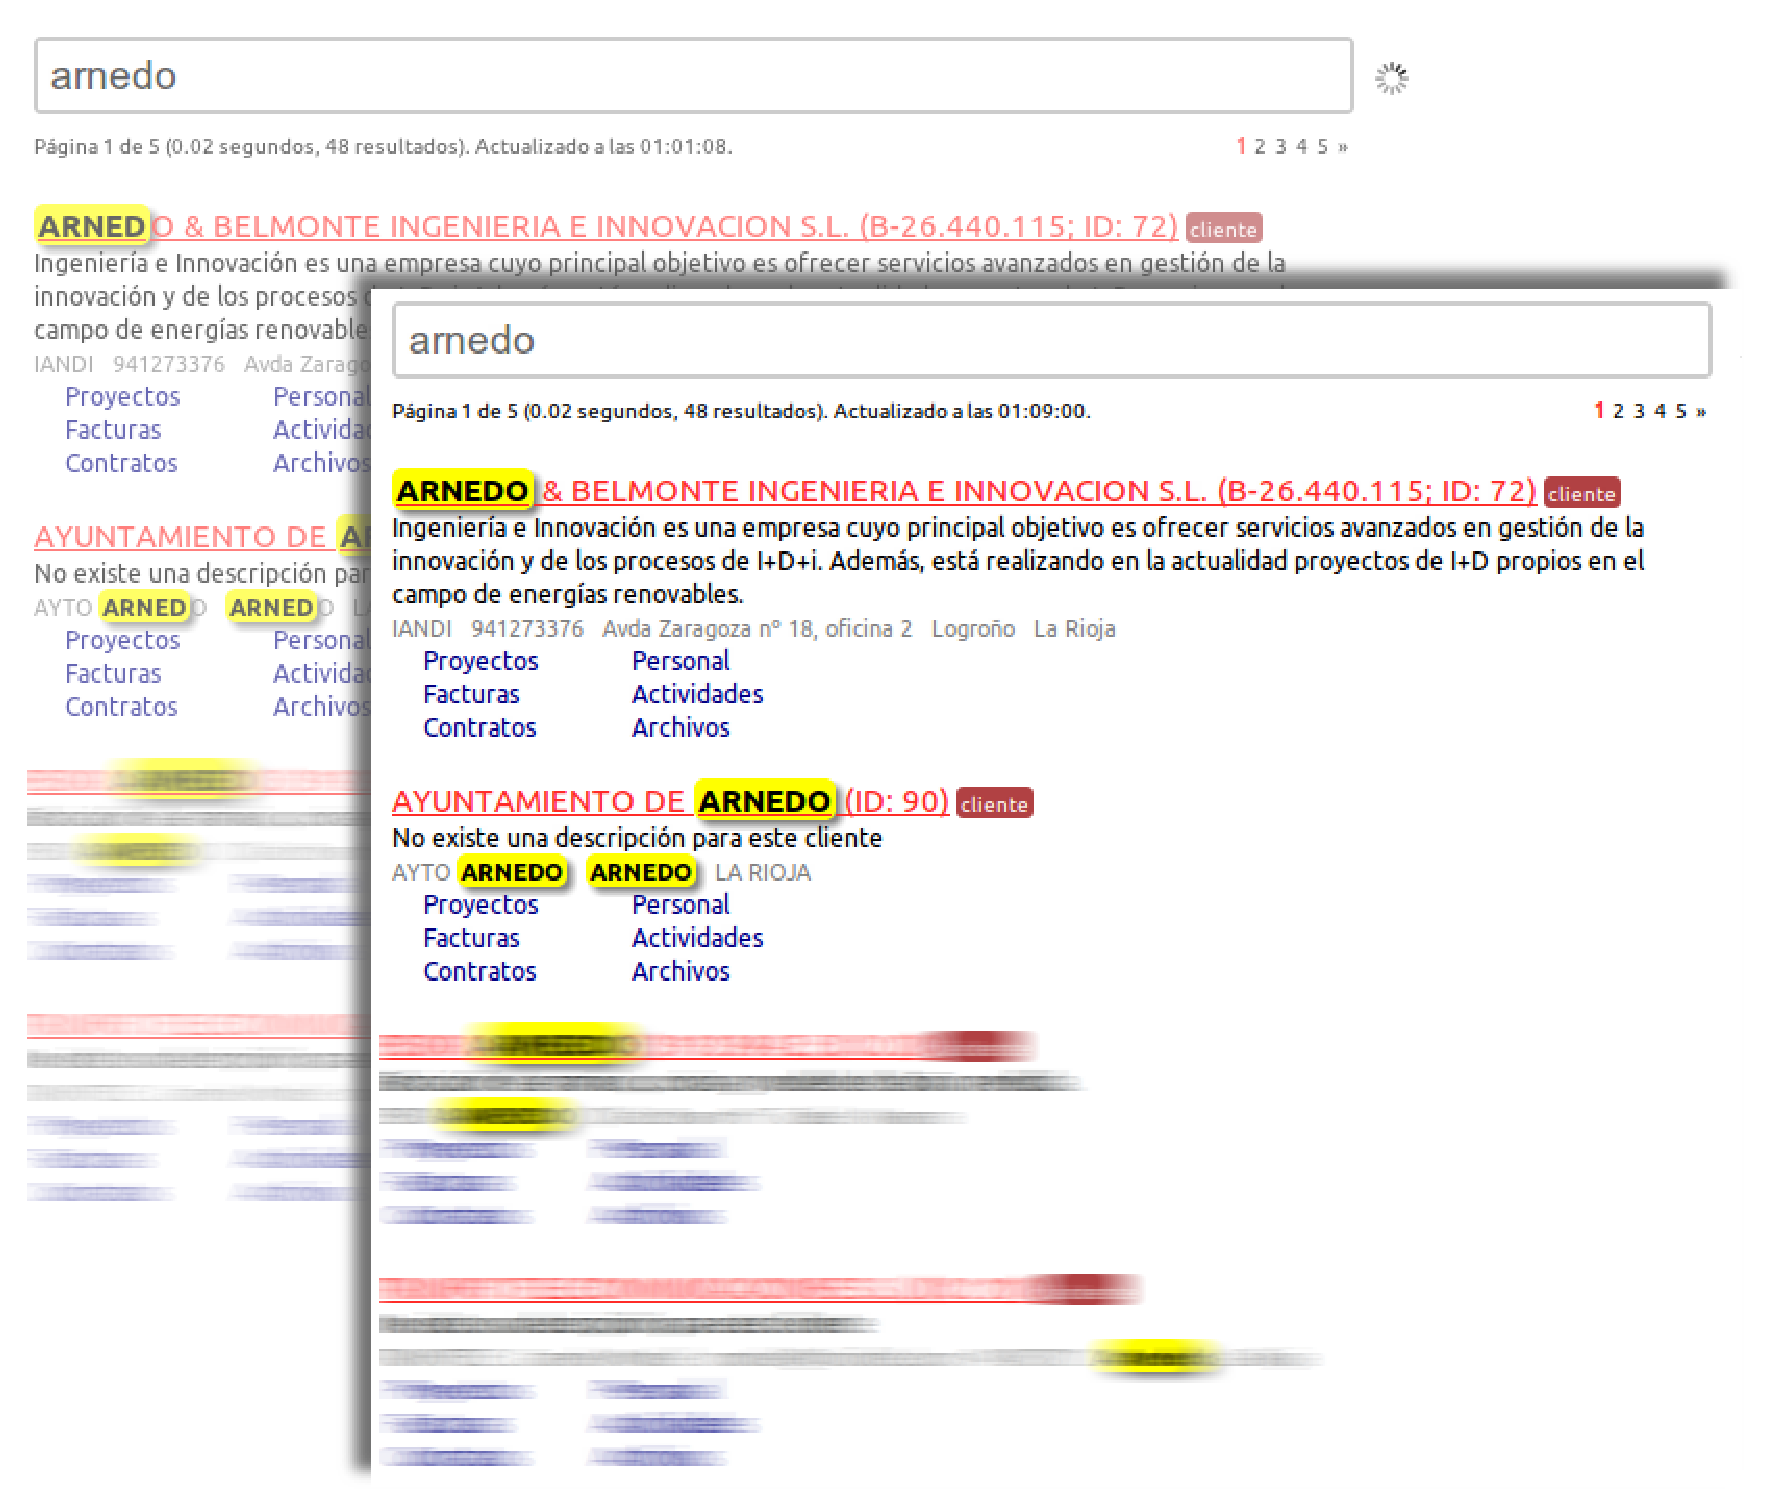
\epsfig{file=imagenes/buscador_cargando.eps,width=5.28in}
\caption{Buscador cargando (izq.) y estado normal (dcha.)}
\label{fig:buscador_cargando}
\end{figure}

La última característica que requiere mención especial es que se permite la
navegación por teclado, de modo que la flecha derecha ($\rightarrow$) pasa a la
siguiente página y la flecha izquierda ($\leftarrow$), a la anterior.

\section{Diseño de la base de datos}

Como ya se ha mencionado anteriormente, se ha empleado una base de datos
relacional gestionada por MySQL. En esta sección, pueden encontrarse los
detalles acerca de las entidades, sus atributos, y las relaciones que se
establecen entre ellas.

Debe notarse que si bien se ha intentado hacer un diseño razonable que no
utilice recursos innecesarios, no se ha llevado a cabo un proceso de
normalización. En los siguientes párrafos se explicará brevemente
la motivación y las decisiones tomadas acerca de los aspectos más relevantes
relacionados con el diseño de la base de datos.

\subsection{Diagrama Entidad/Relación}

En el diagrama de Entidad/Relación (figura \ref{fig:ERD}) puede verse de forma
rápida las entidades involucradas y la forma en que se relacionan entre ellas.
Se han incluido las entidades preexistentes PROYECTO y CLIENTE, ya que
están relacionadas con las nuevas entidades que introduce la herramienta que nos
ocupa. Nótese que, por simplicidad, no se han incluido en este diagrama los
atributos que registran la creación y modificación de los datos.

\begin{figure}
\centering
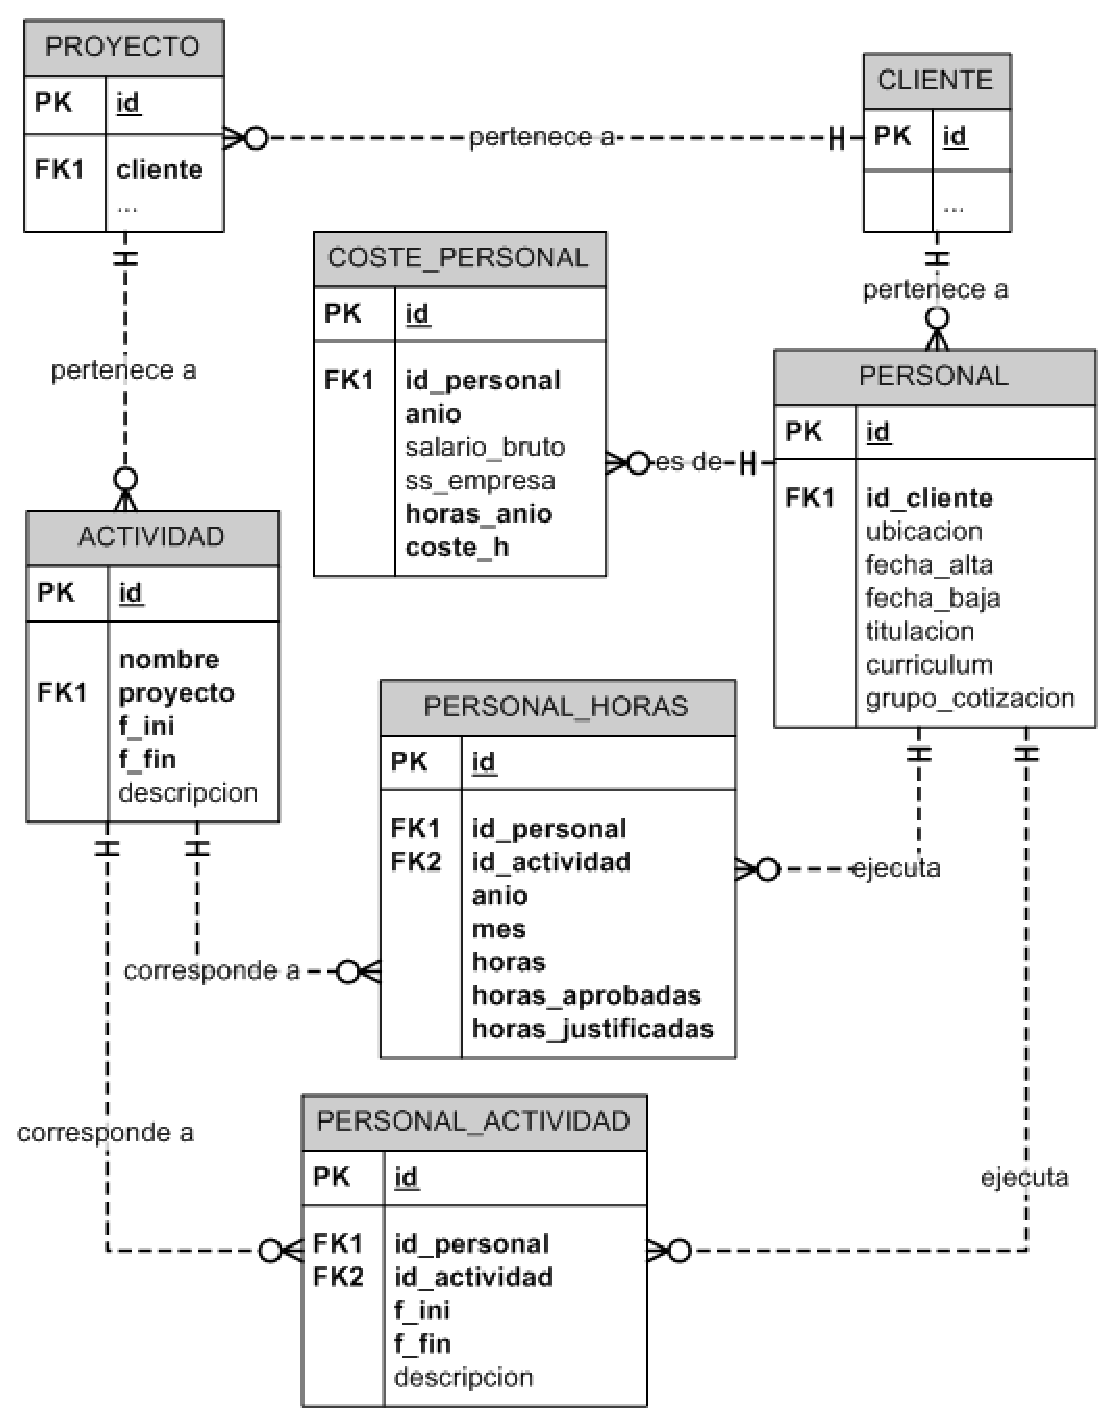
\epsfig{file=imagenes/ERD.eps,width=5.28in}
\caption{Diagrama E--R}
\label{fig:ERD}
\end{figure}

\subsection{Entidades y atributos}

En el cuadro \ref{tab:tablas_atributos} se muestra un resumen de las nuevas
entidades creadas.

Nótese que algunos atributos hacen referencia a entidades preexistentes, como se
explicará en la sección \ref{sec:relaciones}.

\begin{table}
\small
\centering
\begin{tabular}{|l|p{3in}|}\hline
\textbf{Nombre} & \textbf{Atributos}\\\hline\hline
\textbf{ACTIVIDAD} & id, nombre,
    proyecto, f\_ini, f\_fin, descripcion, fecha\_creacion, usu\_creacion,
    fecha\_modificacion, usu\_modificacion\\\hline
\textbf{COSTE\_PERSONAL} & id, id\_personal, anio, salario\_bruto, ss\_empresa,
    coste\_h, horas\_anio, usuario\_creacion, fecha\_creacion, usuario\_act,
    fecha\_act\\\hline
\textbf{PERSONAL} & id, id\_cliente, ubicacion, nombre, fecha\_alta,
    fecha\_baja,    titulacion, curriculum, grupo\_cotizacion, fecha\_creacion,
    usu\_creacion,    fecha\_modificacion, usu\_modificacion \\\hline
\textbf{PERSONAL\_ACTIVIDAD} & id, id\_personal, id\_actividad, f\_ini, f\_fin,
    descripcion, fecha\_creacion, usu\_creacion, fecha\_modificacion,
    usu\_modificacion \\\hline
\textbf{PERSONAL\_HORAS} & id, id\_personal, id\_actividad, anio, mes, horas,
    horas\_aprobadas, horas\_justificadas, fecha\_creacion, usu\_creacion,
    fecha\_modificacion, usu\_modificacion \\\hline
\end{tabular}
\caption{Atributos de las entidades creadas}
\label{tab:tablas_atributos}
\end{table}

La tabla ACTIVIDAD (cuadro \ref{tab:tabla_actividad}) recogerá la información
relacionada con las actividades: su nombre, a qué proyecto pertenecen, fechas
de inicio y finalización y descripción. De manera automática, se recogerán
datos relativos a la creación y modificación de las actividades, de manera que,
en caso de errores o inconsistencias, se pueda recuperar cuándo se produjeron y
quién la introdujo para facilitar la corrección.

\begin{table}
\small
\centering
\begin{tabular}{|l|p{2in}|l|l|}\hline
\textbf{Atributo} & \textbf{Descripción} & \textbf{Tipo de dato} &
\textbf{Nulo} \\\hline\hline
id & identificador autoincremental & INT(11) & No\\\hline
nombre & nombre de la actividad & VARCHAR(255) & No\\\hline
proyecto & identificador del proyecto al que pertenece & INT(11) & No\\\hline
f\_ini & fecha de inicio aproximada & INT(11) & No\\\hline
f\_fin & fecha de fin aproximada & INT(11) & No\\\hline
descripcion & descripcion extensa & TEXT & Sí\\\hline
fecha\_creacion & registro automático de la fecha de creación & INT(11) &
No\\\hline
usuario\_creacion & registro automático del usuario creador & INT(11) &
No\\\hline
fecha\_modificacion & registro automático de la fecha de creación & INT(11) &
Sí\\\hline
usuario\_modificacion & registro automático del usuario modificador & INT(11) &
Sí\\\hline
\end{tabular}
\caption{Atributos de la tabla ACTIVIDAD}
\label{tab:tabla_actividad}
\end{table}

La tabla PERSONAL (cuadro \ref{tab:tabla_personal}) recogerá la información
relacionada con los empleados: su nombre, a qué cliente corresponden,
ubicación, fechas de alta y baja (si procede), titulación, currículum y grupo
de cotización. Las fechas de alta y baja no se han considerado obligatorias
debido a la falta de información al respecto que existe en muchos casos. Si se
conocen, la aplicación será capaz de detectar inconsistencias generadas de la
imputación de horas fuera de esas fechas. Idealmente, los clientes
proporcionarían toda la información relativa a los empleados, pero esto no es lo
común. Como en el caso anterior, se recogerán datos relativos a la creación y
modificación.

\begin{table}
\small
\centering
\begin{tabular}{|l|p{2in}|l|l|}\hline
\textbf{Atributo} & \textbf{Descripción} & \textbf{Tipo de dato} &
\textbf{Nulo} \\\hline\hline
id & identificador autoincremental & INT(11) & No\\\hline
id\_cliente & identificador del cliente al que hace referencia & INT(11) &
No\\\hline
ubicacion & CC.AA. en la que realiza su trabajo & INT(11) & Sí\\\hline
fecha\_alta & fecha de alta en la empresa & INT(11) & Sí\\\hline
fecha\_baja & fecha de baja en la empresa & INT(11) & Sí\\\hline
titulacion & titulación del empleado & VARCHAR(255) & Sí\\\hline
curriculum & currículum resumido del empleado & TEXT & Sí\\\hline
grupo\_cotizacion & grupo de cotización del empleado & VARCHAR(50) & Sí\\\hline
fecha\_creacion & registro automático de la fecha de creación & INT(11) &
No\\\hline
usuario\_creacion & registro automático del usuario creador & INT(11) &
No\\\hline
fecha\_modificacion & registro automático de la fecha de creación & INT(11) &
Sí\\\hline
usuario\_modificacion & registro automático del usuario modificador & INT(11) &
Sí\\\hline
\end{tabular}
\caption{Atributos de la tabla PERSONAL}
\label{tab:tabla_personal}
\end{table}

La tabla COSTE\_PERSONAL (cuadro \ref{tab:tabla_coste_personal}) recogerá la
información relacionada con los registros anuales. El nombre hace referencia al
coste hora del empleado porque este es uno de los datos fundamentales que van a
cambiar anualmente. Se guardan datos relativos al año al que se refiere el
registro, el salario bruto, el coste de Seguridad Social a cargo de la empresa
y el número de horas del convenio. Nótese que del salario bruto, el coste de
Seguridad Social a cargo de la empresa y las horas del convenio, se deduce el
coste hora del empleado, pero de nuevo, es muy común que en un principio no se
conozcan todos estos datos, o se proporcione solo alguno de ellos junto con el
coste hora final. En un caso ideal, podríamos prescindir del campo coste\_hora,
que sería deducido del resto. Como en los casos anteriores, se recogerán datos
relativos a la creación y modificación.

\begin{table}
\small
\centering
\begin{tabular}{|l|p{2in}|l|l|}\hline
\textbf{Atributo} & \textbf{Descripción} & \textbf{Tipo de dato} &
\textbf{Nulo} \\\hline\hline
id & identificador autoincremental & INT(11) & No\\\hline
id\_personal & identificador del empleado al que hace referencia & INT(11) &
No\\\hline
anio & año del registro anual & SMALLINT(4) & No\\\hline
salario\_bruto & salario bruto del empleado en el año & FLOAT(8,2) & Sí\\\hline
ss\_empresa & seguridad social a cargo de la empresa & FLOAT(8,2) & Sí\\\hline
horas\_anio & horas anuales según convenio & SMALLINT(4) & No\\\hline
coste\_h & coste por hora del empleado & FLOAT(4,2) & No\\\hline
fecha\_creacion & registro automático de la fecha de creación & INT(11) &
No\\\hline
usuario\_creacion & registro automático del usuario creador & INT(11) &
No\\\hline
fecha\_modificacion & registro automático de la fecha de creación & INT(11) &
Sí\\\hline
usuario\_modificacion & registro automático del usuario modificador & INT(11) &
Sí\\\hline
\end{tabular}
\caption{Atributos de la tabla COSTE\_PERSONAL}
\label{tab:tabla_coste_personal}
\end{table}

La tabla PERSONAL\_ACTIVIDAD (cuadro \ref{tab:tabla_personal_actividad})
recogerá la información relacionada con las asignaciones de horas realizadas.
Conviene subrayar que es información relacionada con la asignación, no la
asignación misma, ya que no guarda datos de horas. Se ha considerado
interesante conservar esta información, pero no sería estrictamente necesaria
tal y como se ha planteado la solución. En concreto, guarda las fechas exactas
de inicio y finalización del recurso en la actividad, que no tiene por qué
coincidir con las fechas de inicio y finalización de la actividad. Estas fechas
se usan en el reparto de horas, pero no se volverá a tener en cuenta más
adelante. También puede guardar la descripción de la labor del recurso en la
actividad. Se han incluido los datos de creación y modificación por si, en un
futuro, se implementase la capacidad de modificar asignaciones, posibilidad que
ahora es solventada mediante reasignaciones que se sobrescriben.

\begin{table}
\small
\centering
\begin{tabular}{|l|p{2in}|l|l|}\hline
\textbf{Atributo} & \textbf{Descripción} & \textbf{Tipo de dato} &
\textbf{Nulo} \\\hline\hline
id & identificador autoincremental & INT(11) & No\\\hline
id\_personal & identificador del empleado al que hace referencia & INT(11) &
No\\\hline
id\_actividad & identificador de la actividad a la que hace referencia & INT(11)
& No\\\hline
f\_ini & fecha de inicio del empleado en la actividad & INT(11) & No\\\hline
f\_fin & fecha de fin del empleado en la actividad & INT(11) & No\\\hline
descripcion & descripcion de su labor en la actividad & TEXT & Sí\\\hline
fecha\_creacion & registro automático de la fecha de creación & INT(11) &
No\\\hline
usuario\_creacion & registro automático del usuario creador & INT(11) &
No\\\hline
fecha\_modificacion & registro automático de la fecha de creación & INT(11) &
Sí\\\hline
usuario\_modificacion & registro automático del usuario modificador & INT(11) &
Sí\\\hline
\end{tabular}
\caption{Atributos de la tabla PERSONAL\_ACTIVIDAD}
\label{tab:tabla_personal_actividad}
\end{table}

La tabla PERSONAL\_HORAS (cuadro \ref{tab:tabla_personal_horas}) recogerá la
información relacionada con las horas asignadas. Dada la estructura de
concesión de ayudas a la I+D, se necesitan guardar horas presentadas, horas
aprobadas y horas justificadas. Una asignación genera tantos registros como
meses comprenda la duración de la labor del recurso en la actividad, de manera
que, en caso de haber considerado esencial la tabla PERSONAL\_ACTIVIDAD, habría
sido conveniente incluir un campo que hiciera referencia a la asignación a la
que originó cada registro; sin embargo, estos registros van a ser modificables
de manera individual, por lo que se ha decidido relacionar la tabla con el
personal y las actividades directamente. Evidentemente, los registros de esta
tabla están relacionados implícitamente con un solo registro de la tabla
PERSONAL\_ACTIVIDAD por medio de los campos id\_personal e id\_actividad. Como
en casos anteriores, se recogerán datos relativos a la creación y modificación.

\begin{table}
\small
\centering
\begin{tabular}{|l|p{2in}|l|l|}\hline
\textbf{Atributo} & \textbf{Descripción} & \textbf{Tipo de dato} &
\textbf{Nulo} \\\hline\hline
id & identificador autoincremental & INT(11) & No\\\hline
id\_personal & identificador del empleado al que hace referencia & INT(11) &
No\\\hline
id\_actividad & identificador de la actividad a la que hace referencia & INT(11)
& No\\\hline
anio & año al que pertenecen las horas & INT(11) & No\\\hline
mes & año al que pertenecen las horas & INT(11) & No\\\hline
horas & número de horas presentadas & INT(3) & No\\\hline
horas\_aprobadas & registro automático de la fecha de creación & INT(3) &
No\\\hline
horas\_justificadas & registro automático del usuario creador & INT(3) &
No\\\hline
fecha\_creacion & registro automático de la fecha de creación & INT(11) &
No\\\hline
usuario\_creacion & registro automático del usuario creador & INT(11) &
No\\\hline
fecha\_modificacion & registro automático de la fecha de creación & INT(11) &
Sí\\\hline
usuario\_modificacion & registro automático del usuario modificador & INT(11) &
Sí\\\hline
\end{tabular}
\caption{Atributos de la tabla PERSONAL\_HORAS}
\label{tab:tabla_personal_horas}
\end{table}


\subsection{Relaciones}
\label{sec:relaciones}

% \begin{table}
% \footnotesize
{\footnotesize
\noindent\begin{tabular}{|l|p{1.5in}|p{0.40in}|p{0.75in}|}\hline
\textbf{Relación} & \textbf{Descripción} &
\textbf{Ent.}\footnotemark[1] &
\textbf{Atributos} \\\hline\hline
personal\_pertenece\_a\_cliente & cada recurso pertenece únicamente a un cliente
    del sistema & PER \newline CLI & id\_cliente \newline id \\\hline
actividad\_pertenece\_a\_proyecto & cada actividad pertenece únicamente a un
    proyecto del sistema & ACT \newline PRO & proyecto \newline id
    \\\hline
anualidad\_es\_de\_personal & el personal contiene registros para cada año
    & C\_P \newline PER & id\_personal \newline id \\\hline
personal\_ejecuta\_trabajos & el personal realiza actividades durante un
    periodo de tiempo determinado & P\_A \newline PER & id\_personal \newline id
    \\\hline
personal\_ejecuta\_horas & el personal trabaja un número de horas al mes
    determinado & P\_H \newline PER & id\_personal \newline id
    \\\hline
trabajo\_corresponde\_a\_actividad & las actividades son llevadas a cabo
    por medio de las actuaciones de los empleados & P\_A \newline ACT &
    id\_actividad \newline id \\\hline
hora\_corresponde\_a\_actividad & cada conjunto de horas pertenece a una
actividad concreta & P\_H \newline ACT & id\_actividad \newline id
    \\\hline
\end{tabular}
\footnotetext[1]{Entidades |
PER: PERSONAL \quad CLI: CLIENTE \quad ACT: ACTIVIDAD \quad PRO: PROYECTO \quad
C\_P: COSTE\_PERSONAL \quad P\_A: PERSONAL\_ACTIVIDAD \quad P\_H:
PERSONAL\_HORAS}
}

\section{Diseño del sistema}
\label{sec:diseno_del_sistema}

Como se explicó en el capítulo \ref{chp:descripcion}, la arquitectura física del
sistema consiste en un servidor ejecutando sobre Microsoft Windows con una base
de datos MySQL interpretada en el lado del servidor mediante PHP, cuyo código
resultante es gestionado por el servidor web HTTP Apache.

Internamente, la arquitectura está basada en un paradigma imperativo. El
motivo, que también se ha discutido previamente en esta memoria, es la
integración con el resto de la aplicación, desarrollada y mantenida por
Ingenieros Industriales con conocimientos básicos de programación, y cuyo
principal responsable no sigue en la plantilla.

En la parte preexistente, ni siquiera se habían definido apenas funciones, por
lo que parte del código se repetía una y otra vez. Para esta parte de la
herramienta, sí se han definido multitud de funciones, que se han implementado
en el archivo de sesión que se incluye (mediante \textit{include()}) en todas
las páginas, agrupadas por su naturaleza y los módulos a los que se refieren.
Los futuros mantenedores de la herramienta han recibido, como consecuencia,
nociones básicas sobre este nuevo planteamiento.

 
\subsection{Diagramas de secuencia}

Los diagramas de secuencia tratan de mostrar visualmente la interacción entre
dos o más sistemas o entidades. En esta sección, se emplearán de forma básica
para dar una idea más detallada de lo que sucede de forma interna, aspecto que
no se puede apreciar en los casos de uso de la sección \ref{sec:casos_de_uso}.
Los detalles acerca de la implementación se verán en el capítulo
\ref{chp:implementacion}. Se ha creado un diagrama de secuencia para los casos
de uso más interesantes, alternando escenarios de éxito con otros con errores o
mensajes de advertencia.

\begin{figure}
\centering
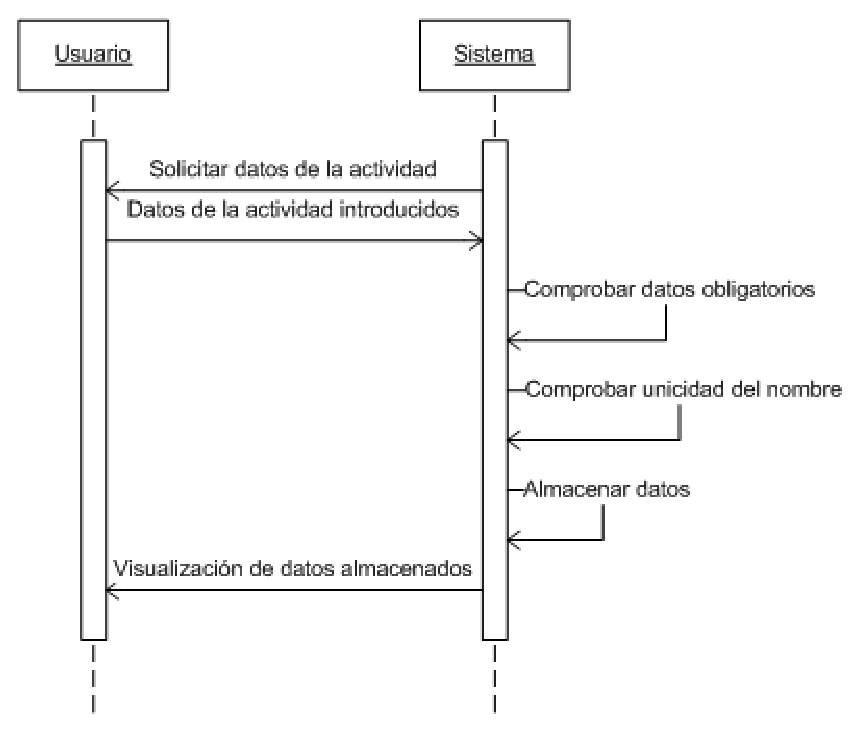
\epsfig{file=imagenes/secuencia/crear_actividad.eps,width=4in}
\caption{Diagrama de secuencia: creación de actividad.}
\label{fig:crear_actividad}
\end{figure}

\begin{figure}
\centering
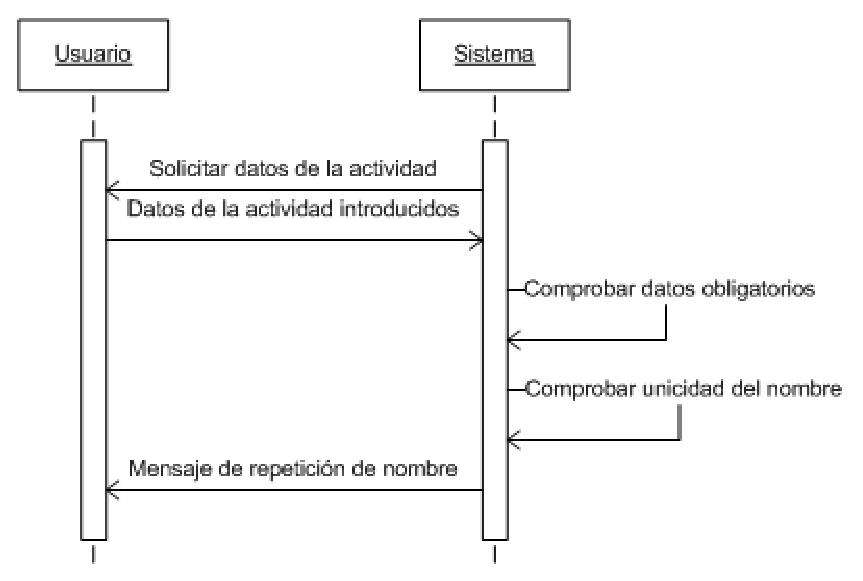
\epsfig{file=imagenes/secuencia/crear_actividad_repetida.eps,width=4in}
\caption{Diagrama de secuencia: creación de actividad con repetición.}
\label{fig:crear_actividad_repetida}
\end{figure}

\begin{figure}
\centering
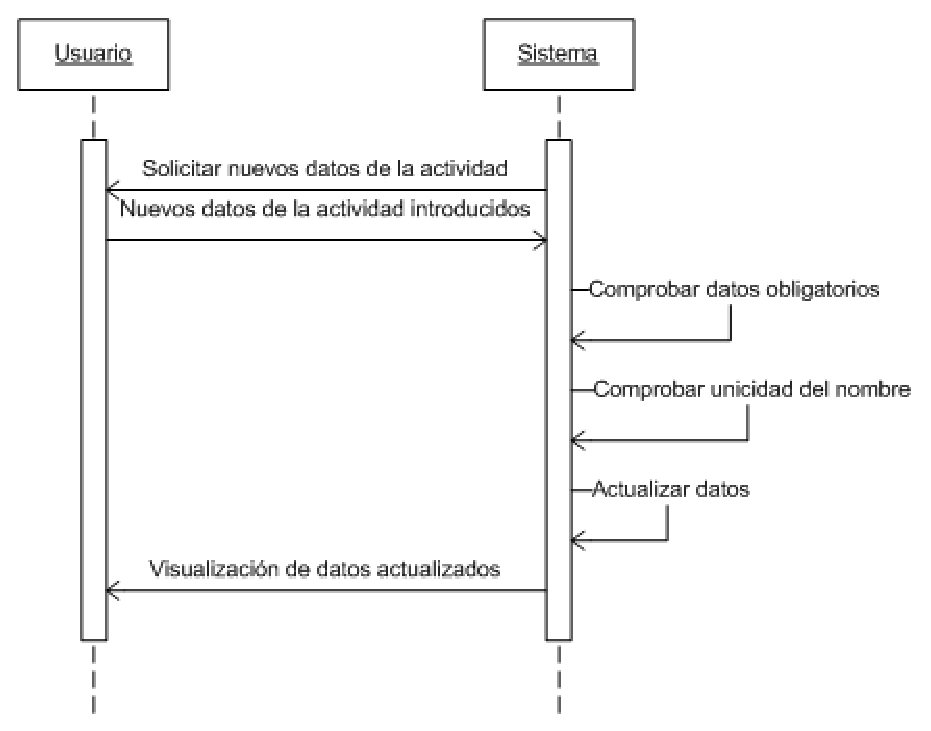
\epsfig{file=imagenes/secuencia/actualizar_actividad.eps,width=4in}
\caption{Diagrama de secuencia: modificación de actividad.}
\label{fig:actualizar_actividad}
\end{figure}

\begin{figure}
\centering
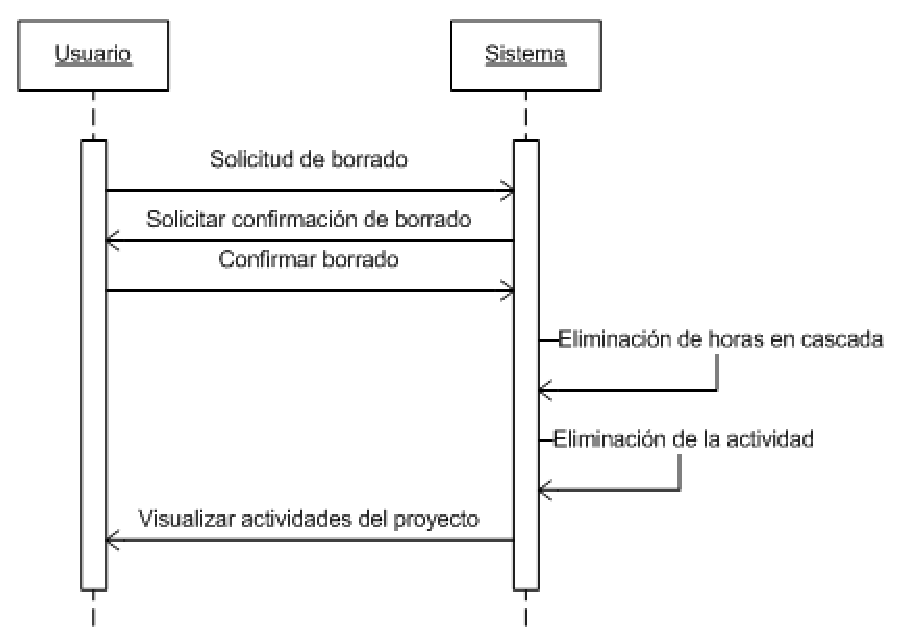
\epsfig{file=imagenes/secuencia/eliminacion_actividad.eps,width=4in}
\caption{Diagrama de secuencia: eliminación de actividad.}
\label{fig:eliminacion_actividad}
\end{figure}

\begin{figure}
\centering
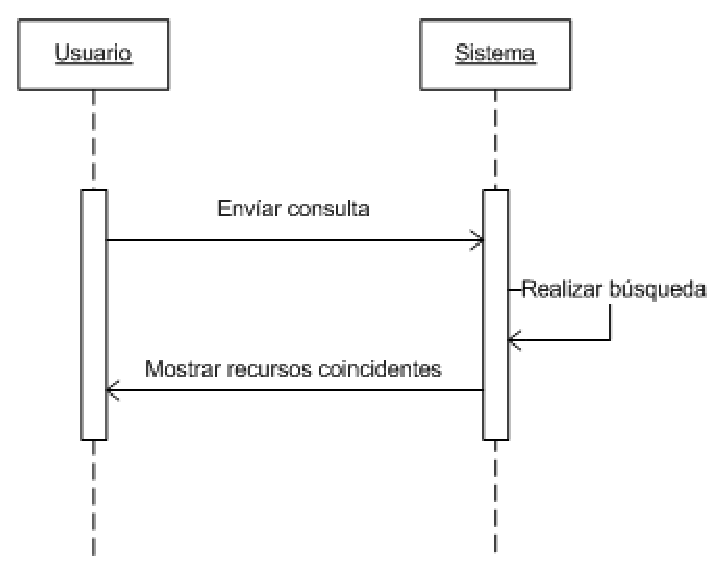
\epsfig{file=imagenes/secuencia/buscar_recurso.eps,width=3.5in}
\caption{Diagrama de secuencia: búsqueda de recurso.}
\label{fig:buscar_recurso}
\end{figure}

\begin{figure}
\centering
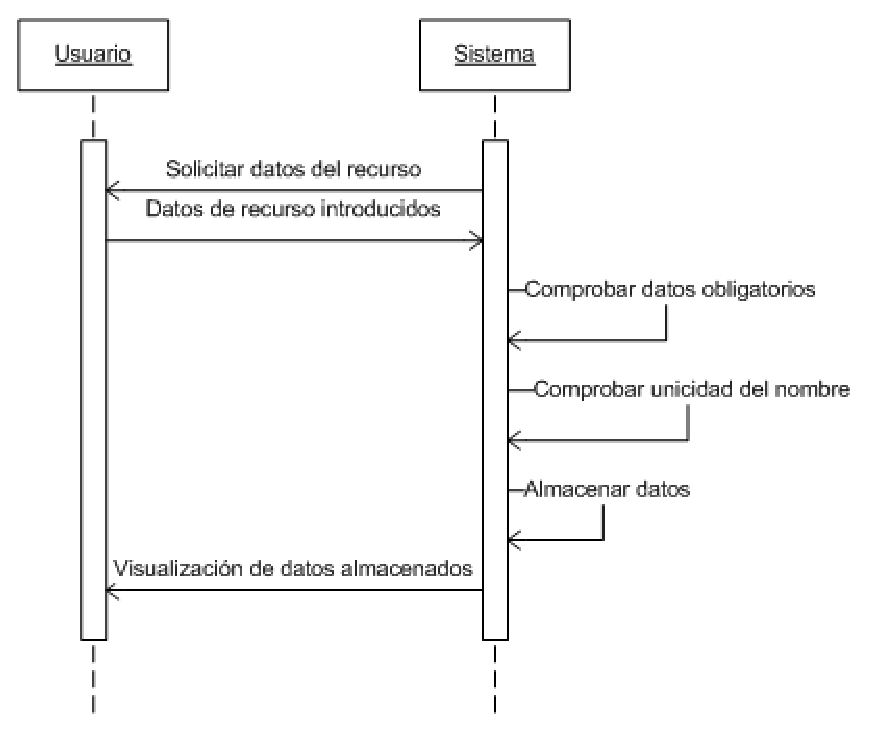
\epsfig{file=imagenes/secuencia/crear_recurso.eps,width=4in}
\caption{Diagrama de secuencia: creación de recurso.}
\label{fig:crear_recurso}
\end{figure}

\begin{figure}
\centering
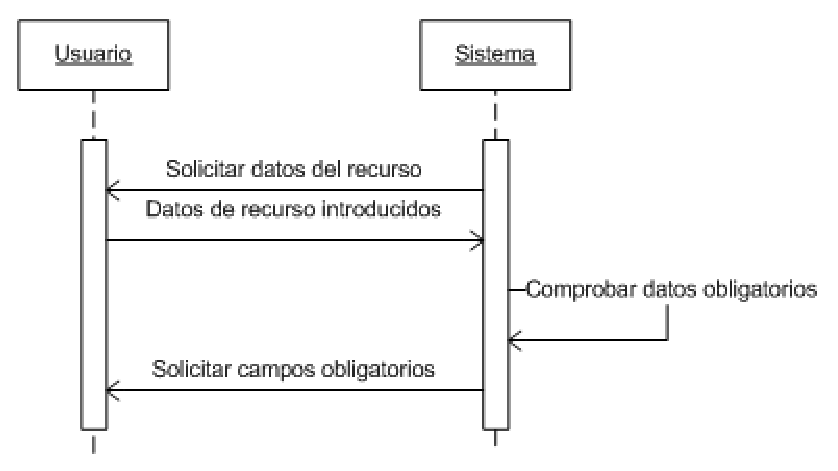
\epsfig{file=imagenes/secuencia/crear_recurso_campos.eps,width=4in}
\caption{Diagrama de secuencia: creación de recurso incompleta.}
\label{fig:crear_recurso_campos}
\end{figure}

\begin{figure}
\centering
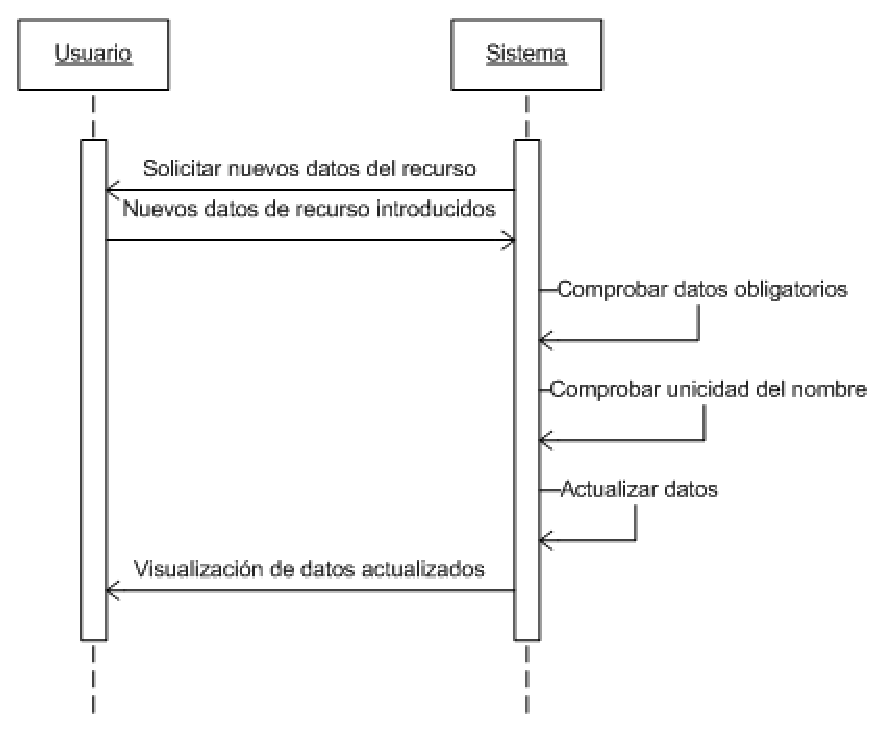
\epsfig{file=imagenes/secuencia/actualizar_recurso.eps,width=4in}
\caption{Diagrama de secuencia: modificación de recurso.}
\label{fig:actualizar_recurso}
\end{figure}

\begin{figure}
\centering
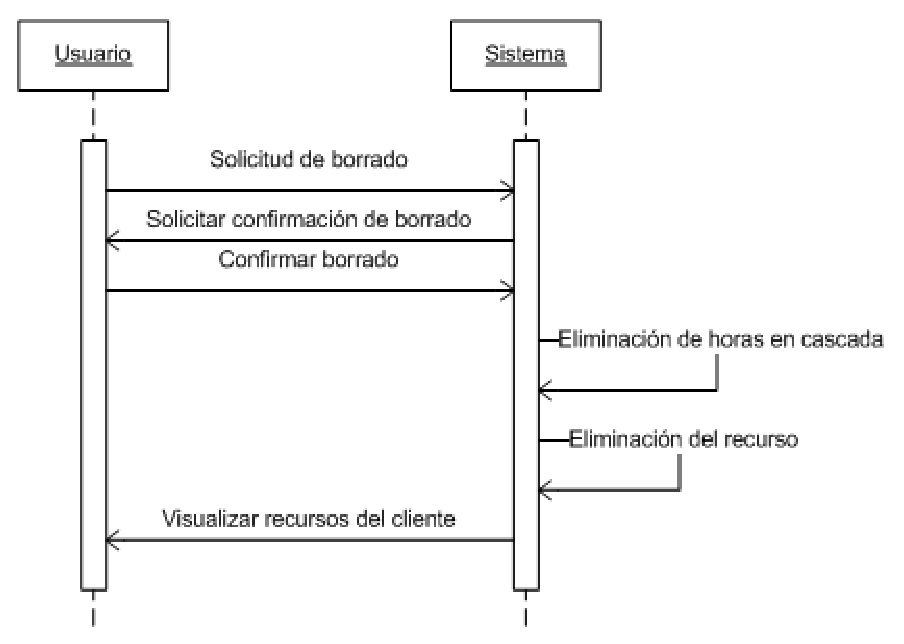
\epsfig{file=imagenes/secuencia/eliminacion_recurso.eps,width=4in}
\caption{Diagrama de secuencia: eliminación de recurso.}
\label{fig:eliminacion_recurso}
\end{figure}

\begin{figure}
\centering
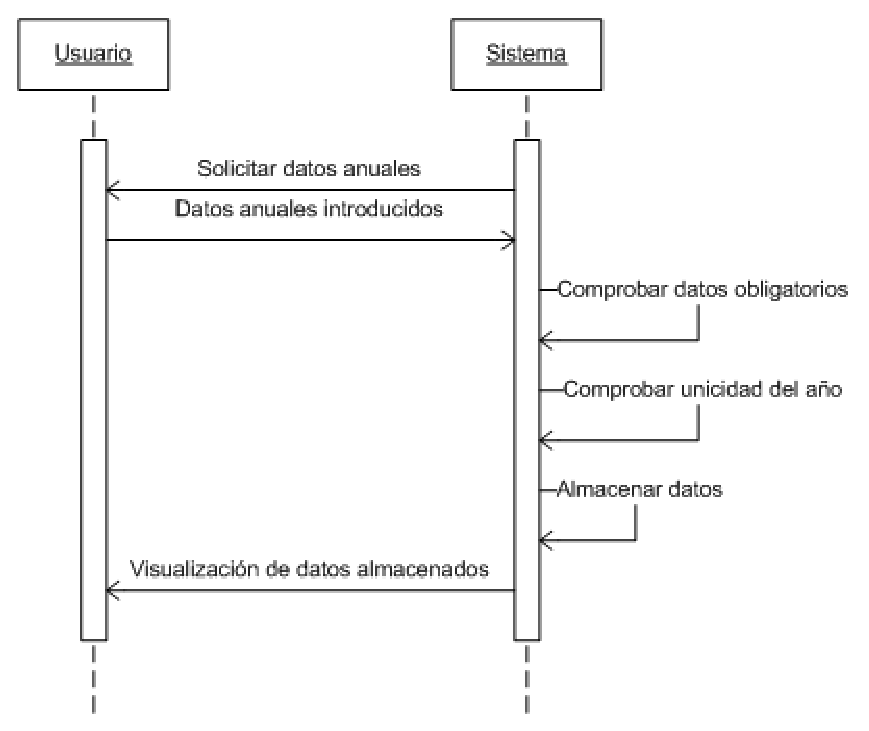
\epsfig{file=imagenes/secuencia/crear_registro_anual.eps,width=4in}
\caption{Diagrama de secuencia: creación de registro anual.}
\label{fig:crear_registro_anual}
\end{figure}

\begin{figure}
\centering
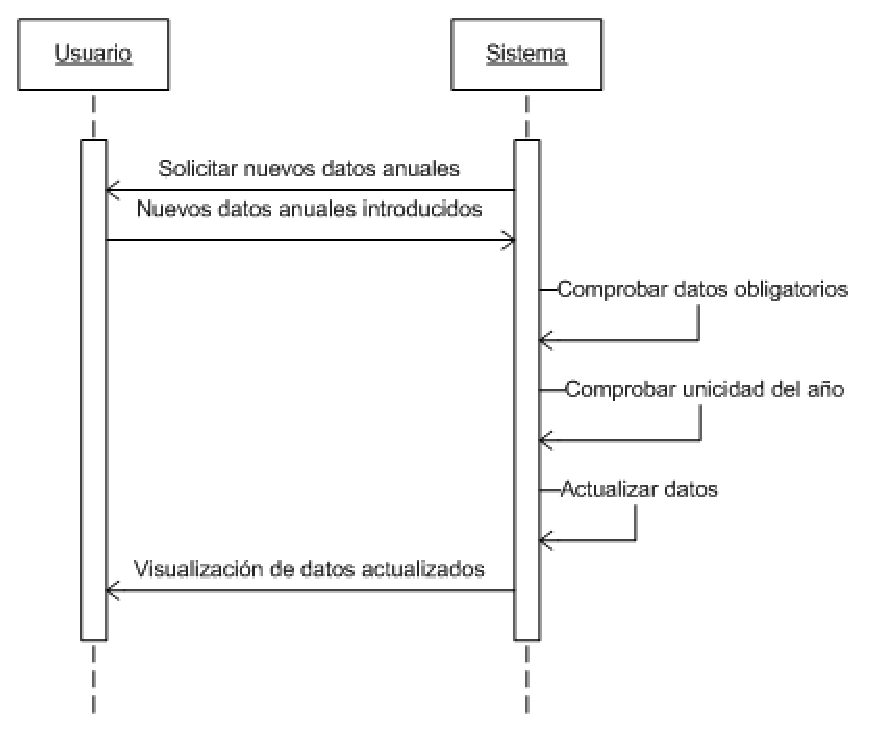
\epsfig{file=imagenes/secuencia/modificar_registro_anual.eps,width=4in}
\caption{Diagrama de secuencia: modificación de registro anual.}
\label{fig:modificar_registro_anual}
\end{figure}

\begin{figure}
\centering
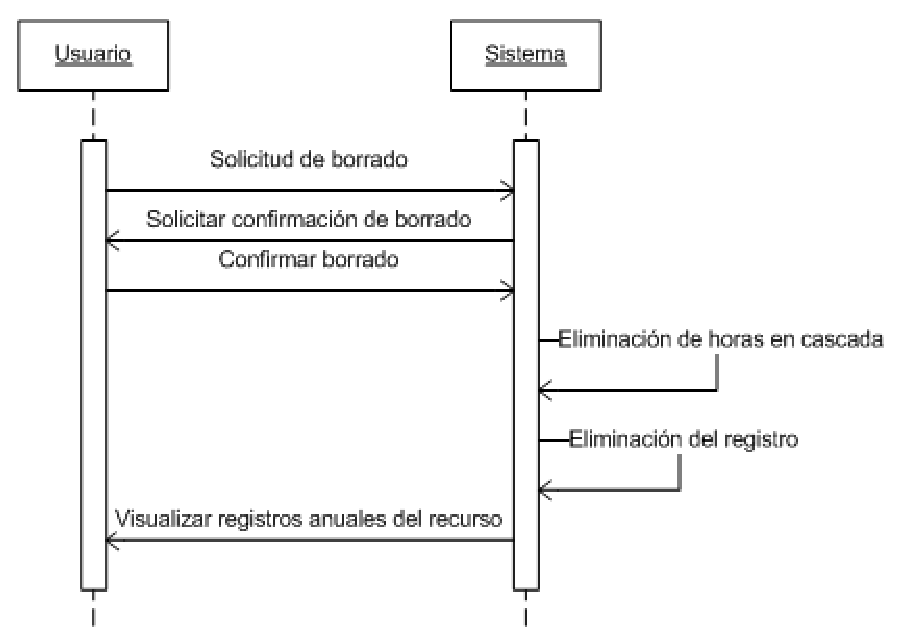
\epsfig{file=imagenes/secuencia/eliminacion_registro.eps,width=4in}
\caption{Diagrama de secuencia: eliminación de registro anual.}
\label{fig:eliminacion_registro}
\end{figure}

\begin{figure}
\centering
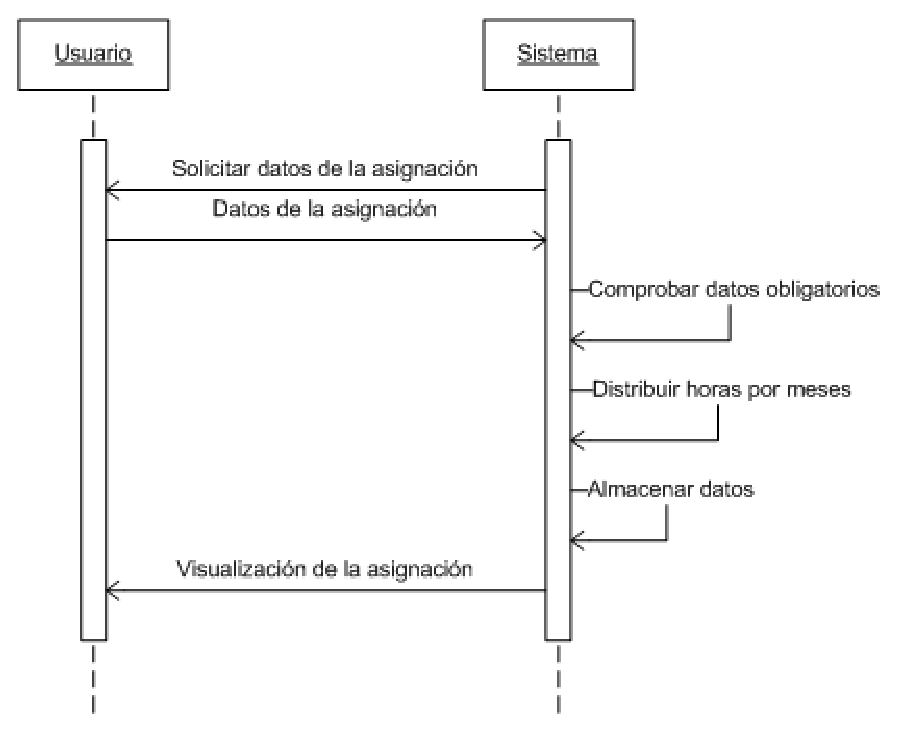
\epsfig{file=imagenes/secuencia/asignacion_horas.eps,width=4in}
\caption{Diagrama de secuencia: asignación de horas.}
\label{fig:asignacion_horas}
\end{figure}

\begin{figure}
\centering
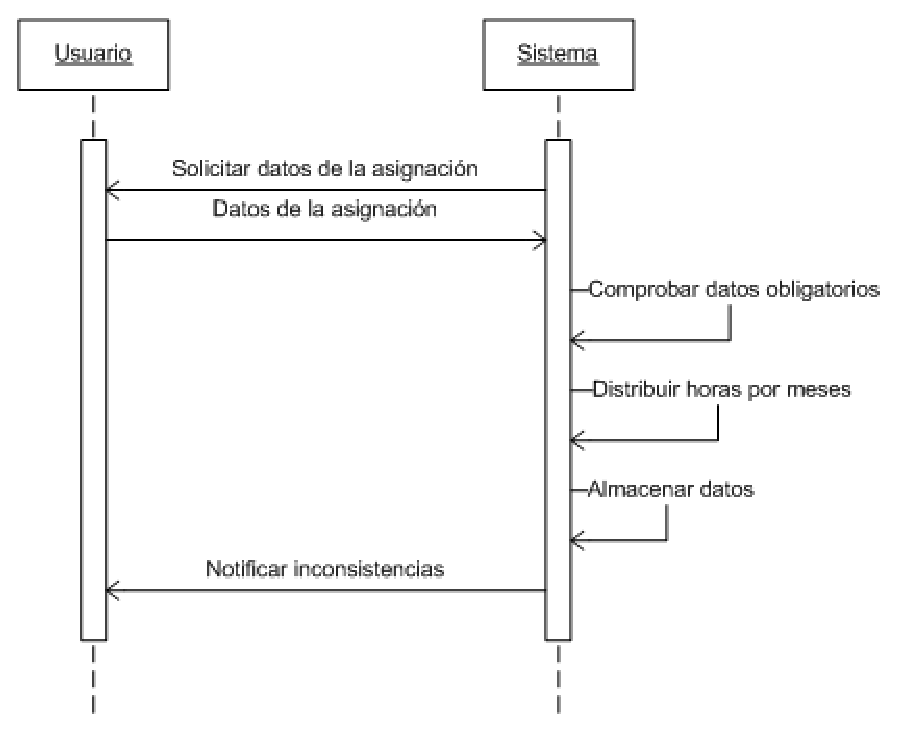
\epsfig{file=imagenes/secuencia/asignacion_horas_inconsistencia.eps,width=4in}
\caption{Diagrama de secuencia: asignación de horas con inconsistencias.}
\label{fig:asignacion_horas_inconsistencia}
\end{figure}



